\chapter{Andreev Bound State Current in SNS-junction}
\label{sec:current}
In chapter \ref{sec:Josephson} we saw how the Josephson current can be expressed in terms of the free energy and phase difference between the two superconductors \eqref{JosephsonCurrent}. In chapter \ref{sec:FreeEnergy} we expressed the free energy in terms of the energy levels, $E_{\kbf}$. Using equation \eqref{JosephsonCurrent} and \eqref{FreeEnergy} we can thus express the Josephson current in terms of the ABS energy and the phase difference:
\begin{equation}
\begin{split}
    I_x(\Delta \varphi) &= \sum_{k_y} \delta I(\fet{r},\fet{k}) \rightarrow \int dy \int \frac{dk_y}{2\pi} \delta I(\fet{r},\fet{k}),\\
    I_y(\Delta \varphi) &= \sum_{k_x} \delta I(\fet{r},\fet{k}) \rightarrow \int dx \int \frac{dk_x}{2\pi} \delta I(\fet{r},\fet{k}),\\
\end{split}
\label{TotalCurrent}
\end{equation}
where we have defined 
\begin{equation}
    \delta I(\fet{r},\fet{k}) \equiv -\frac{2e}{\hbar}\tanh\left(\frac{E_{\kbf}}{2k_BT}\right)\frac{\partial E_{\kbf}}{\partial (\Delta \varphi)}
\label{Current5}
\end{equation}
and $I_y$ should be zero due to current conservation. The current density will be given as
\begin{equation}
\begin{split}
    j_x(x,y) &= \int \frac{dk_y}{2\pi} \delta I(\fet{r},\fet{k}) = \frac{k_F}{2\pi}\int_{-\pi/2}^{\pi/2} d\theta_k \cos\theta_k \delta I(\fet{r},\fet{k}) ,\\
    j_y(x,y) &= \int \frac{dk_x}{2\pi} \delta I(\fet{r},\fet{k}) = \frac{k_F}{2\pi}\int_{-\pi/2}^{\pi/2} d\theta_k \sin\theta_k \delta I(\fet{r},\fet{k}),
\end{split}
\label{CurrentDensity}
\end{equation}
where we have let 
\begin{equation}
\begin{pmatrix}dk_x\\dk_y\end{pmatrix} \rightarrow k_F\begin{pmatrix}\sin\theta_k\\ \cos\theta_k\end{pmatrix}d\theta_k
\end{equation}
as we consider the circular Fermi surface, as stated in chapter \ref{sec:PhysicalSystem}.
\\
\\
In chapter \ref{sec:energies} the ABS energy levels were found for the three different situations and we will in this chapter use these energies in equation \eqref{CurrentDensity} to find the current density and in equation \eqref{TotalCurrent} to find the total and critical current for each of the three situations. For the analytical progress we will consider the high temperature regime, $(k_BT \gtrsim \Delta_0)$, in which the analytical calculations are simpler.

\section{ABS current without barriers or applied field}
\label{sec:CurrentWithout}
In the case with no barriers or magnetic field we use equation \eqref{AndreevEnergy1} in equation \eqref{Current5} to obtain
\begin{equation}
    \delta I = \frac{e\Delta_0}{\hbar}\sin\left(\frac{\Delta\varphi}{2}\right)\tanh\left(\frac{\Delta_0\cos(\Delta\varphi/2)}{2k_BT}\right),
\end{equation}
which we notice is independent of the trajectory of the particle. From equation \eqref{CurrentDensity} one finds the current density to be zero in the $y$-direction, $j_y(x,y) = 0$, and uniform in the $x$-direction, $j_x(x,y) = I_x/W$, where $W$ is the junction width (indicated in figure \ref{fig:Explaination}) and $I_x$ as the total current:
\begin{equation}
\begin{split}
   I_x = k_F W\frac{e\Delta_0}{\pi \hbar} \sin\left(\frac{\Delta\varphi}{2}\right)\tanh\left(\frac{\Delta_0\cos(\Delta\varphi/2)}{2k_BT}\right).
\end{split}
\label{TotalCurrent}
\end{equation}
In the high temperature regime $(k_BT \gtrsim \Delta_0)$ this can be approximated to
\begin{equation}
    I_x = k_F W\frac{e\Delta_0}{\pi \hbar} \sin\left(\frac{\Delta\varphi}{2}\right)\frac{\Delta_0\cos(\Delta\varphi/2)}{2k_BT} = I_{c,0}\sin \Delta \varphi
\label{WithoutField}
\end{equation}
with 
\begin{equation}
    I_{c,0} = \frac{k_F W e\Delta_0^2}{4\pi \hbar k_BT}
\label{Ic0-highT}
\end{equation}
as the high temperature critical current. These results are well known !!!CITE!!! and will be used for comparison in the preceding sections. 

\section{ABS current with barriers}
\label{sec:CurrentWithBarriers}
The ABS energy levels in the case of no barriers was found in equation \eqref{AndreevEnergy2}. Inserting this in equation \eqref{Current5} yields
\begin{equation}
\delta I = \frac{e \Delta_0}{2 \hbar}\frac{\sin(\Delta \varphi)}{\sqrt{(\cos^2(\Delta \varphi /2 )+ \zeta)(\zeta + 1)}}\tanh\left(\frac{\Delta_0}{2k_BT}\sqrt{\frac{\cos^2(\Delta \varphi/2) + \zeta}{\zeta + 1}}\right).
\end{equation}
Also here $\delta I $ is independent of the trajectory such that the current density is uniform. The total current is
\begin{equation}
I_x = k_FW \frac{e \Delta_0}{2 \pi \hbar}\frac{\sin(\Delta \varphi)}{\sqrt{(\cos^2(\Delta \varphi /2 )+ \zeta)(\zeta + 1)}}\tanh\left(\frac{\Delta_0}{2k_BT}\sqrt{\frac{\cos^2(\Delta \varphi/2) + \zeta}{\zeta + 1}}\right).
\end{equation}
The high temperature critical current is
\begin{equation}
I_{c,\zeta} = \frac{k_F W e\Delta_0^2}{4\pi \hbar k_BT}\frac{1}{\zeta + 1} = \frac{I_{c,0}}{\zeta+1},
\end{equation}
with $I_{c,0}$ is the critical current without barriers \eqref{Ic0-highT}. Figure \ref{fig:CurrentWithoutField} shows how the total current varies with the phase difference, $\Delta \varphi$, in the high temperature regime ($k_BT = \Delta_0$) for different barrier strengths, $\zeta$.
\begin{figure}[hhh]
\centering
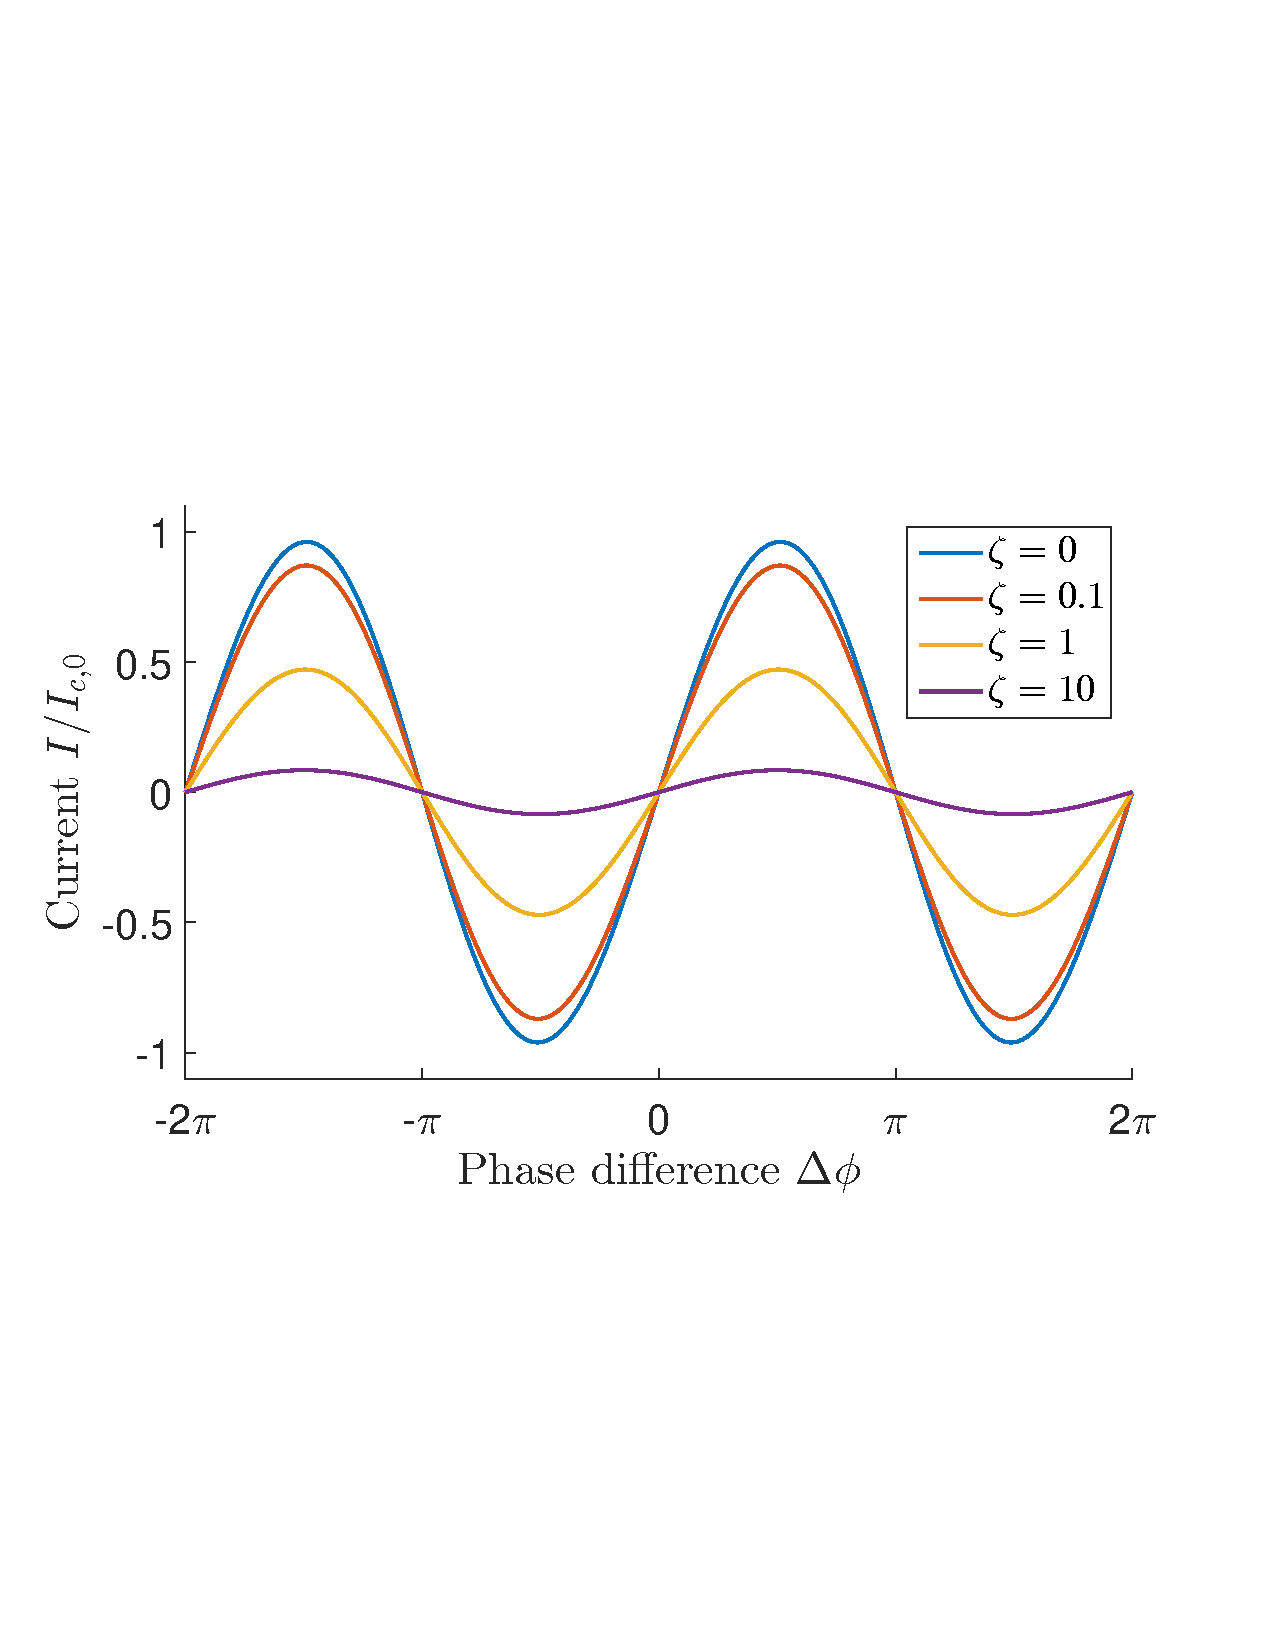
\includegraphics[width=10cm,clip=true,trim=0cm 8cm 1.5cm 9cm]{fig/WithoutField}
\caption{blabla}
\label{fig:CurrentWithoutField}
\end{figure}

\section{ABS current with applied field}
\label{sec:CurrentWithB}
With no barriers, but magnetic field we find the current from the ABS energy in equation \eqref{AndreevEnergy3}:
\begin{equation}
    \delta I_k(\Delta \varphi) = \frac{e\Delta_0}{\hbar} \sin\left(\frac{\Delta \varphi}{2} - \frac{\gamma_k}{2}\right)\tanh\left(\frac{\Delta_0\cos\left(\frac{\Delta \varphi}{2} - \frac{\gamma_k}{2}\right)}{2k_BT}\right)
\label{dIwithB}
\end{equation}
which in the high temperature regime ($k_BT \gtrsim \Delta_0$), can be approximated to
\begin{equation}
    \delta I_k(\Delta \varphi) \approx \frac{e\Delta_0^2}{4\hbar k_BT} \sin\left(\Delta \varphi -\gamma_k\right).
\label{dIwithBHighT}
\end{equation}
We notice that this expression is maximized when
\begin{equation}
    \gamma_k = \frac{4n-3}{2}\pi+\Delta\varphi
\label{Maximize}
\end{equation}
with $n$ as an integer. The Aharonov-Bohm phase shift, $\gamma_k$, will depend on the modulation and strength of the magnetic field, and on the trajectory of the particle. We will here consider three different modulations of the magnetic field. That is a uniform magnetic field (section \ref{sec:ConstField}), sinusoidal field varying along the junction (section \ref{sec:alongJunction}) and sinusoidal field varying along the interfaces (section \ref{sec:alongInterface}). 
\\
\\
The magnetic field will be expelled in the superconducting region, due to the Meissner effect. We assume the penetration depth to be short even in the high-field regime, i.e. when $l_m \lesssim L$ with with $l_m = \sqrt{\hbar/eB}$ as the magnetic length. The Lorentz effect will change the trajectories in the magnetic field into arcs of cyclotron radius $l_{\mathrm{cycl}} = \hbar k_F / eB = k_F l_m^2$. However, we assume that $k_F L$ is sufficiently large such that $l_{\mathrm{cycl}}/L = k_FL(l_m/L)^2 \gg 1$ for the fields considered and we can neglect the curvature of the trajectories. 

\subsection{Uniform magnetic field}
\label{sec:ConstField}
We will first consider a uniform magnetic field of strength $B$:
\begin{equation}
    \fet{B} = B\left[\Theta(x+L/2) - \Theta(x-L/2) \right]\hat{z},
\end{equation}
and choose the gauge of the $\fet{A}$-field as
\begin{equation}
    \fet{A} = -By\left[\Theta(x+L/2) - \Theta(x-L/2) \right]\hat{x}.
\end{equation}
The Aharonov-Bohm phase shift, $\gamma(x_0,y_0,\theta_k)$, is calculated from equation \eqref{gamma} by integration along a path through the point $(x_0,y_0)$ at an angle $\theta_k$ with the $x$-axis, as shown in figure \ref{fig:Explaination}. The trajectory will be given by the line
\begin{equation}
    y(x) = y_0-x_0\tan\theta_k + x\tan\theta_k.
    \label{trajectory}
\end{equation}
Using this in equation \eqref{gamma} we find the phase shift:
\begin{equation}
    \gamma = -\frac{2e}{\hbar}\int_L^R \fet{A}\cdot d\fet{l} = B\frac{2e}{\hbar}\int_{-L/2}^{L/2}y(x)dx = \frac{2L}{l_m^2}\left(y_0 - x_0\tan\theta_k \right).
\label{gamma1}
\end{equation}
%If we assume $W$ to be much larger than $L$ we can ignore the boundaries along the junction, and the current will be conserved such that there will be no $x_0$ dependence. 
This expression is used in equation \eqref{dIwithB} and \eqref{CurrentDensity} in order to find the current density. The result from numerical computation is shown in figure \ref{fig:Constant} for three different magnetic lengths revealing the appearance of a row of current vortex-antivortex pairs. From equation \eqref{Maximize} the current density is found to be maximum at $x_0=0$ (at which the phase shift is $\theta_k$-independent) and
\begin{equation}
    y_0 = \frac{l_m^2}{L}\left(\frac{4n-3}{4}\pi + \frac{\Delta \varphi}{2}\right).
\end{equation}
Hence, the vortex lattice constant (the distance between two vortices) is
\begin{equation}
    a_{\mathrm{vortex}} = \pi\frac{l_m^2}{L}.
\end{equation}
Figure \ref{fig:Constant} shows how the vortex lattice constant increases with the magnetic length. In the resutl we have tken the phase difference to be $\Delta \varphi = \pi/2$, however, the pattern looks identical for any $\Delta \varphi$.
\begin{figure}[hhh]
\centering
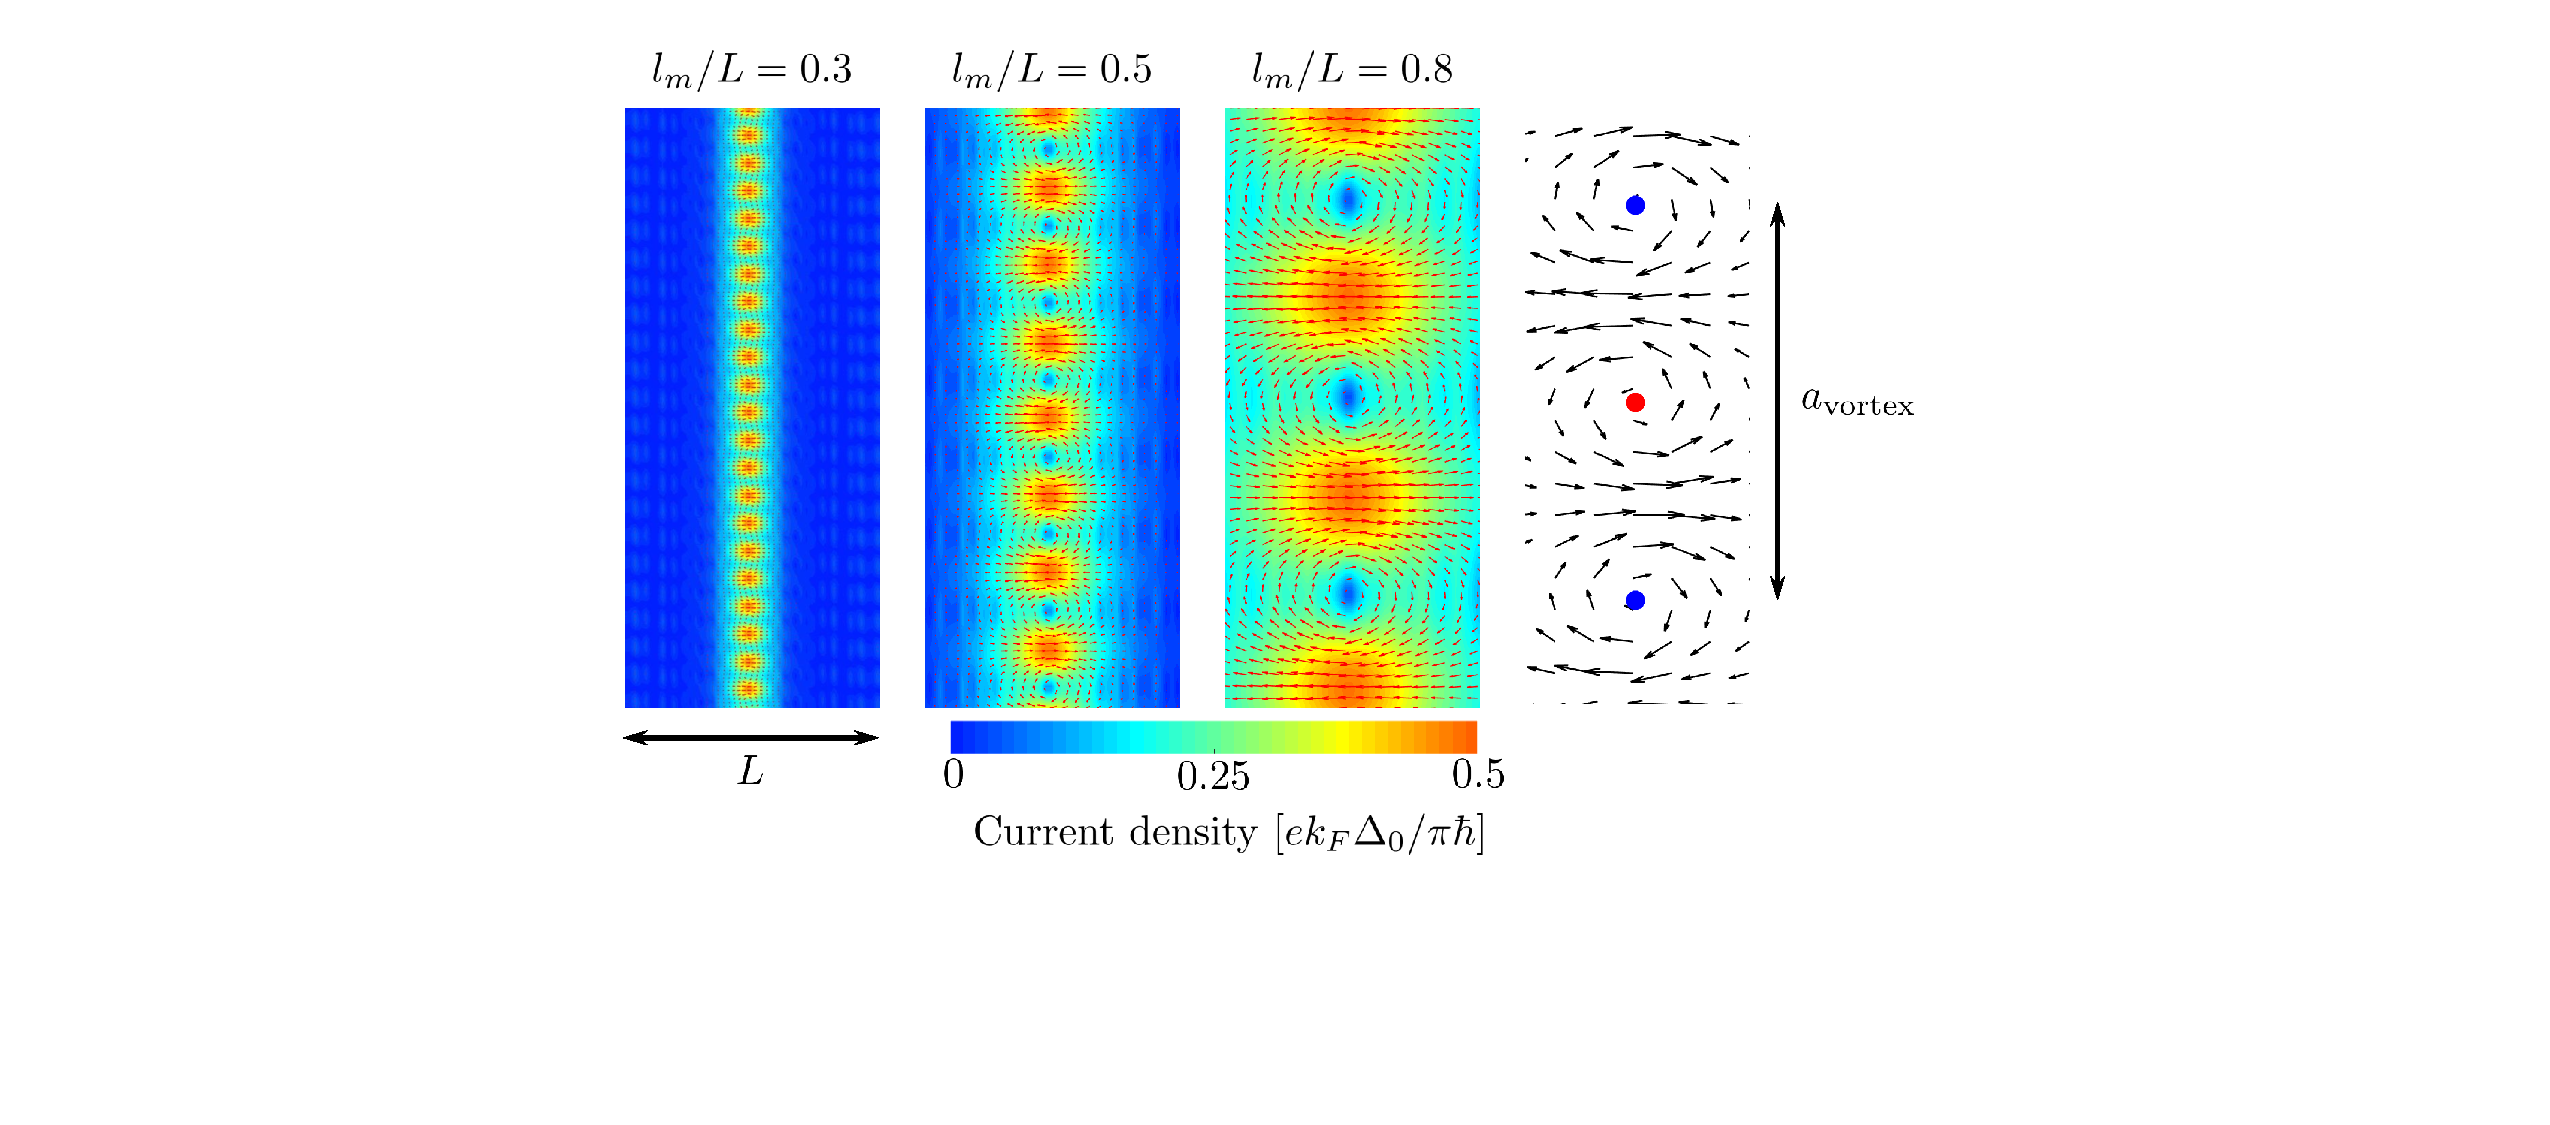
\includegraphics[width=15cm,clip=true,trim=10cm 4cm 10cm 0cm]{fig/Dist1}
%\subfigure[]{\includegraphics[width=3.9cm]{Dustin}\label{fig:Dustin}}
%\hfill
%\subfigure[]{\includegraphics[width=3.45cm]{Martin}\label{fig:Martin}}
\caption{blabla}
\label{fig:Constant}
\end{figure}
\\
\\
In order to find the total current we combine equation \eqref{TotalCurrent}, \eqref{CurrentDensity} and \eqref{dIwithB}:
\begin{equation}
I_x = \frac{k_F}{2\pi}\frac{e\Delta_0}{\hbar}\int_{-W/2}^{W/2}dy_0\int_{-\pi/2}^{\pi/2}d\theta_k\cos \theta_k \sin\left(\frac{\Delta \varphi}{2}-\frac{\gamma}{2}\right)\tanh\left(\frac{\Delta_0}{2k_BT}\cos\left(\frac{\Delta \varphi}{2}-\frac{\gamma}{2}\right)\right)
\end{equation}
which in the high temperature regime $(k_BT \gtrsim \Delta_0)$ is simplified to
\begin{equation}
I_x = \frac{I_{c,0}}{2W}\int_{-W/2}^{W/2}dy_0\int_{\pi/2}^{\pi/2} d\theta_k \cos \theta_k \sin (\Delta \varphi - \gamma ).
\label{TotalCurrentHighT}
\end{equation}
From equation \eqref{gamma1} we notice that $\gamma(x_0,y_0,\theta_k) = -\gamma(x_0,-y_0,-\theta)$ which allows us to write
\begin{equation}
I_x = \frac{I_{c,0}}{W}\sin(\Delta \varphi) \int_{-W/2}^{W/2}dy_0\int_0^{\pi/2} d\theta_k\cos \theta_k \cos\gamma.
\end{equation}
The integral over $y_0$ gives
\begin{equation}
\int_{-W/2}^{W/2}dy_0\cos\gamma = \frac{l_m^2}{L}\sin\left(\frac{LW}{l_m^2}\right)\cos\left(\frac{2L}{l_m^2}x_0\tan\theta_k\right) \approx \frac{l_m^2}{L}\sin\left(\frac{LW}{l_m^2}\right),
\end{equation}
where we the last equality is taken in the low field regime $(l_m \gg L)$ in order to simplify the analytical expression. The total current is thus
\begin{equation}
I_x = I_{c,0}\frac{\sin\left(\frac{e}{\hbar}\Phi\right)}{\frac{e}{\hbar}\Phi}\sin \Delta \varphi
\end{equation}
with $\Phi = BLW$ as the magnetic flux and we find the critical current at $\Delta \varphi = \pi/2$:
\begin{equation}
I_{c,\mathrm{const}} = I_{c,0} \left|\frac{\sin\left(\frac{e}{\hbar}\Phi\right)}{\frac{e}{\hbar}\Phi}\right|
\end{equation}
which is the well known Fraunhofer oscillations. The critical current resulting from numerical calculations is shown in figure \ref{fig:Fraunhofer}.
\begin{figure}[hhh]
\centering
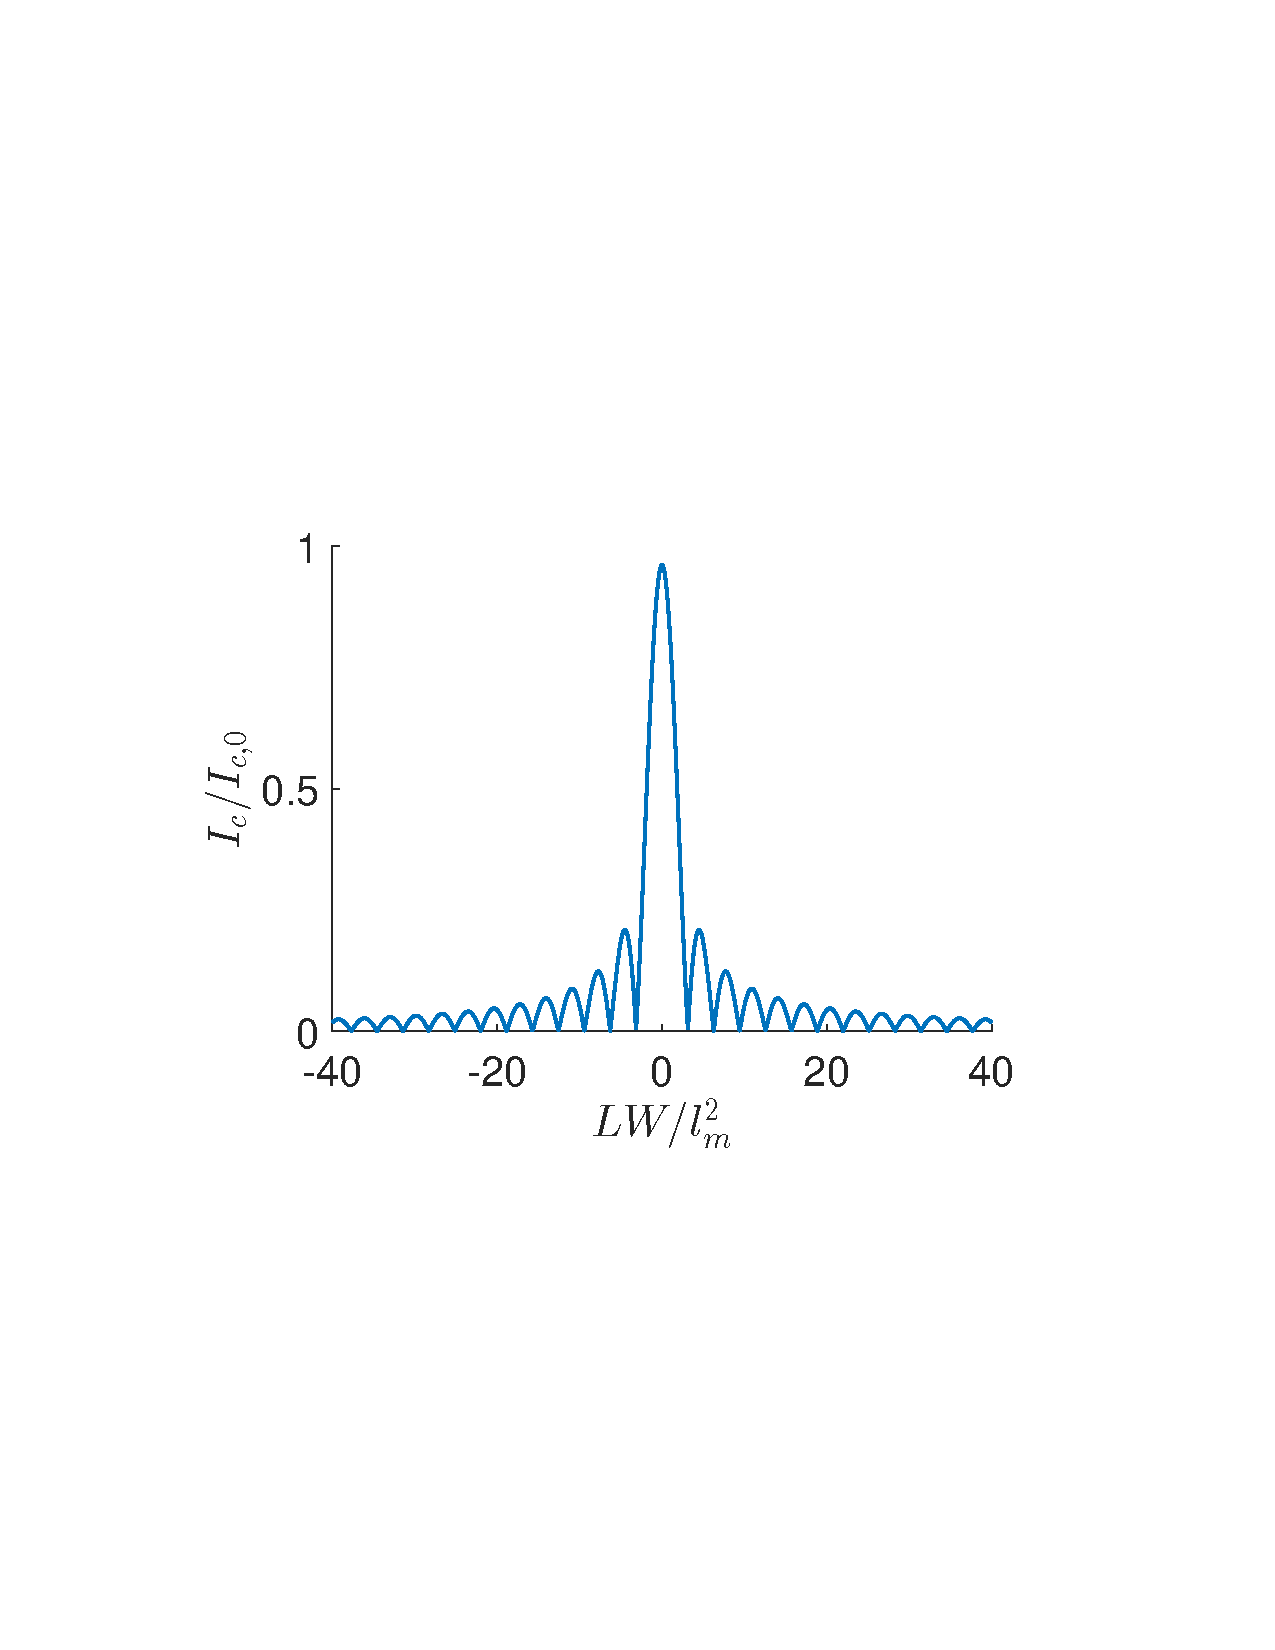
\includegraphics[width=10cm,clip=true,trim=3cm 8cm 3cm 8cm]{fig/Critical1}
%\subfigure[]{\includegraphics[width=3.9cm]{Dustin}\label{fig:Dustin}}
%\hfill
%\subfigure[]{\includegraphics[width=3.45cm]{Martin}\label{fig:Martin}}
\caption{blabla}
\label{fig:Fraunhofer}
\end{figure}
\\
\subsection{Sinusoidal field varying along the junction}
\label{sec:alongJunction}
We will next consider a sinusoidal magnetic field along the junction:
\begin{equation}
    \fet{B} = B\sin\left(\frac{2\pi}{\lambda}x + \varphi\right)\left[\Theta(x+L/2) - \Theta(x-L/2) \right]\hat{z}
\label{B4}
\end{equation}
with the gauge
\begin{equation}
    \fet{A} = -By\sin\left(\frac{2\pi}{\lambda}x + \varphi\right)\left[\Theta(x+L/2) - \Theta(x-L/2) \right]\hat{x}.
\label{A4}
\end{equation}
Again we use \eqref{gamma} and integrate along the trajectory in \eqref{trajectory} to find the Aharonov-Bohm phase shift:
\begin{equation}
\begin{split}
    \gamma &= \frac{2}{l_m^2}\int_{-L/2}^{L/2}y(x)\sin\left(\frac{2\pi}{\lambda} +\varphi \right) dx \\
    &= \frac{2\lambda}{\pi l_m^2}\left(\left[y_0 - x_0\tan\theta_k\right]\sin\left(\frac{\pi L}{\lambda}\right)\sin\varphi+\frac{L}{2}\tan\theta_k\left[\frac{\lambda}{\pi L}\sin\left(\frac{\pi L}{\lambda}\right)-\cos\left(\frac{\pi L}{\lambda}\right)\right]\cos\varphi\right).
\end{split}
\label{gamma2}
\end{equation}


\subsubsection{Symmetric field}
More specifically we let $\varphi = \pi/2$ in \eqref{B4} so that the the magnetic field becomes symmetric about the $y$-axis and the second term in equation \eqref{gamma2} is zero such that the phase shift is
\begin{equation}
\gamma= \frac{2\lambda}{\pi l_m^2}\left[y_0 - x_0\tan\theta_k\right]\sin\left(\frac{\pi L}{\lambda}\right) = \gamma_{\mathrm{uni}}\frac{\sin\left(\pi L/\lambda\right)}{\pi L/\lambda}
\label{Gamma5}
\end{equation}
where $\gamma_{\mathrm{uni}}$ is the Aharonov-Bohm phase shift in the uniform magnetic field as given in equation \eqref{gamma1}. As this expression is proportional to the phase shift for uniform field we expect appearance of current vortices, but with a vortex lattice constant dependent on the wavelength of the magnetic field: 
\begin{equation}
    a_{\mathrm{vortex}} = \pi\frac{l_m^2}{L}\frac{\pi L/\lambda}{\sin(\pi L/\lambda)}.
\end{equation}
Hence, the distance between the vortices can be controlled not only by changing the magnetic field strength, but also by changing the wavelength of the symmetric field. For wavelengths $\lambda = L/n$, with $n$ as an non-zero integer, we notice that $a_{\mathrm{vortex}} \rightarrow \infty$ and $\gamma \rightarrow 0$, such that we expect the vortices to vanish and the current to be unaffected by the magnetic field.
\\
\\
We can use $\gamma$ \eqref{Gamma5} in equation \eqref{dIwithB} and \eqref{CurrentDensity} to calculate the current density numerically. The result is shown in figure \ref{fig:Dist5} for three different wavelengths. We see how the distance between the vortices is changed when the wavelength of the magnetic field is changed, and theat for some wavelengths, e.g. $\lambda = L/2$, the vortices vanish. The fact that the supercurrent survives for arbitrarily large field strengths, $B$, as long as the spacial modulation wavelengths satisfy $\lambda = L/n$ is remarkable and is one of the key findings in this thesis.
\begin{figure}[hhh]
\centering
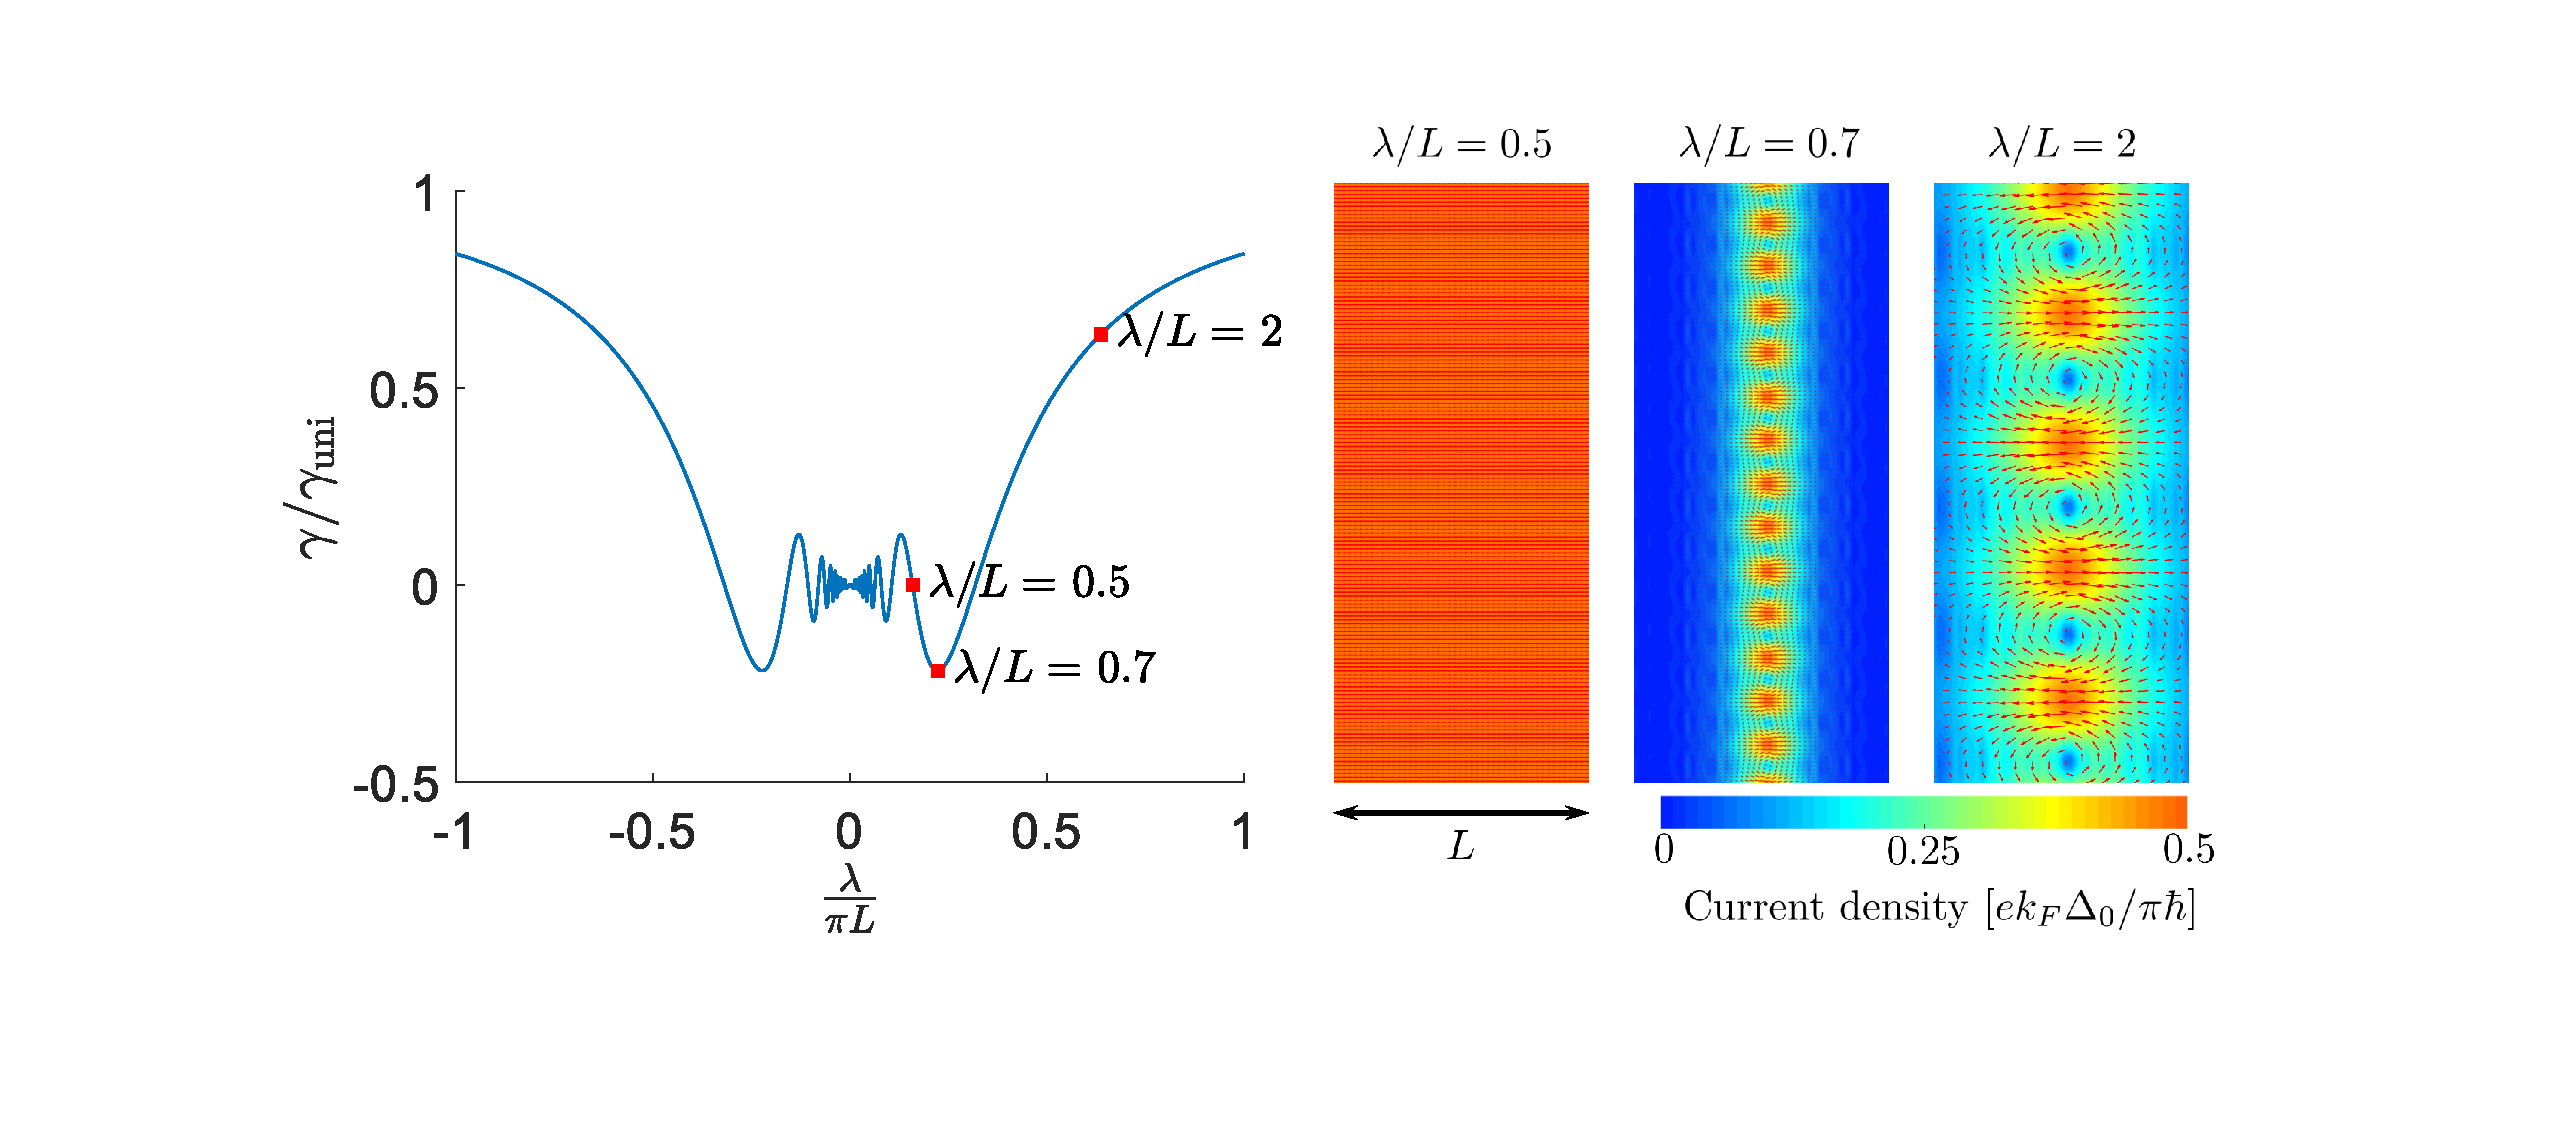
\includegraphics[width=17cm,clip=true,trim=5cm 3cm 4.4cm 2cm]{fig/Dist5}
%\subfigure[]{\includegraphics[width=3.9cm]{Dustin}\label{fig:Dustin}}
%\hfill
%\subfigure[]{\includegraphics[width=3.45cm]{Martin}\label{fig:Martin}}
\caption{blabla}
\label{fig:Dist5}
\end{figure}
\\
\\
The total current is found in the same manner as in section  \ref{sec:ConstField}, giving
\begin{equation}
I_x = 
%I_{c,0}\sin(\Delta \varphi)\frac{\sin\left(\frac{LW}{l_m^2}\frac{\sin(\pi L/\lambda)}{\pi L/\lambda}\right)}{\frac{LW}{l_m^2}\frac{\sin(\pi L/\lambda)}{\pi L/\lambda}} =
I_{c,0}\sin\Delta\varphi\frac{\sin(\frac{e}{\hbar}\Phi)}{\frac{e}{\hbar}\Phi}
\end{equation}
where $\Phi$ is the magnetic flux:
\begin{equation}
    \Phi = \int \fet{B}\cdot d\fet{A} = 
    %\int \int B\cos\left(\frac{2\pi}{\lambda}x\right)dxdy = 
    \Phi_{\mathrm{uni}}\frac{\sin(\pi L/\lambda)}{\pi L/\lambda},
\end{equation}
with $\Phi_{\mathrm{uni}} = BWL$ as the magnetic flux in the uniform field. In terms of magnetic flux this expression is identical to the total current in the uniform field. However, the flux, and consequently the total and critical current, will be dependent on the wavelength. The high temperature critcal current will be given as 
\begin{equation}
    I_c = I_{c,0}\left|\frac{\sin\left(\frac{LW}{l_m^2}\frac{\sin(\pi L/\lambda)}{\pi L/\lambda}\right)}{\frac{LW}{l_m^2}\frac{\sin(\pi L/\lambda)}{\pi L/\lambda}}\right|.
\end{equation}
In figure \ref{fig:Critical5} the critical current obtained from numerical computation is shown for different wavelengths, $\lambda$, and varying magnetic field strength, $B$. We recognize the Fraunhofer pattern as we had for the uniform field, but the decay can be controlled by changing the wavelength, $\lambda$, and for some wavelengths, e.g. $\lambda = L/2$, the critical current maintains constant regardless of the field strength. We propose that this can be understood as an interference phenomenon where the phase-shift picked up by the electrons and holes comprising the ABS level are completely cancelled out due to the specific magnetic field profile.
\begin{figure}[hhh]
\centering
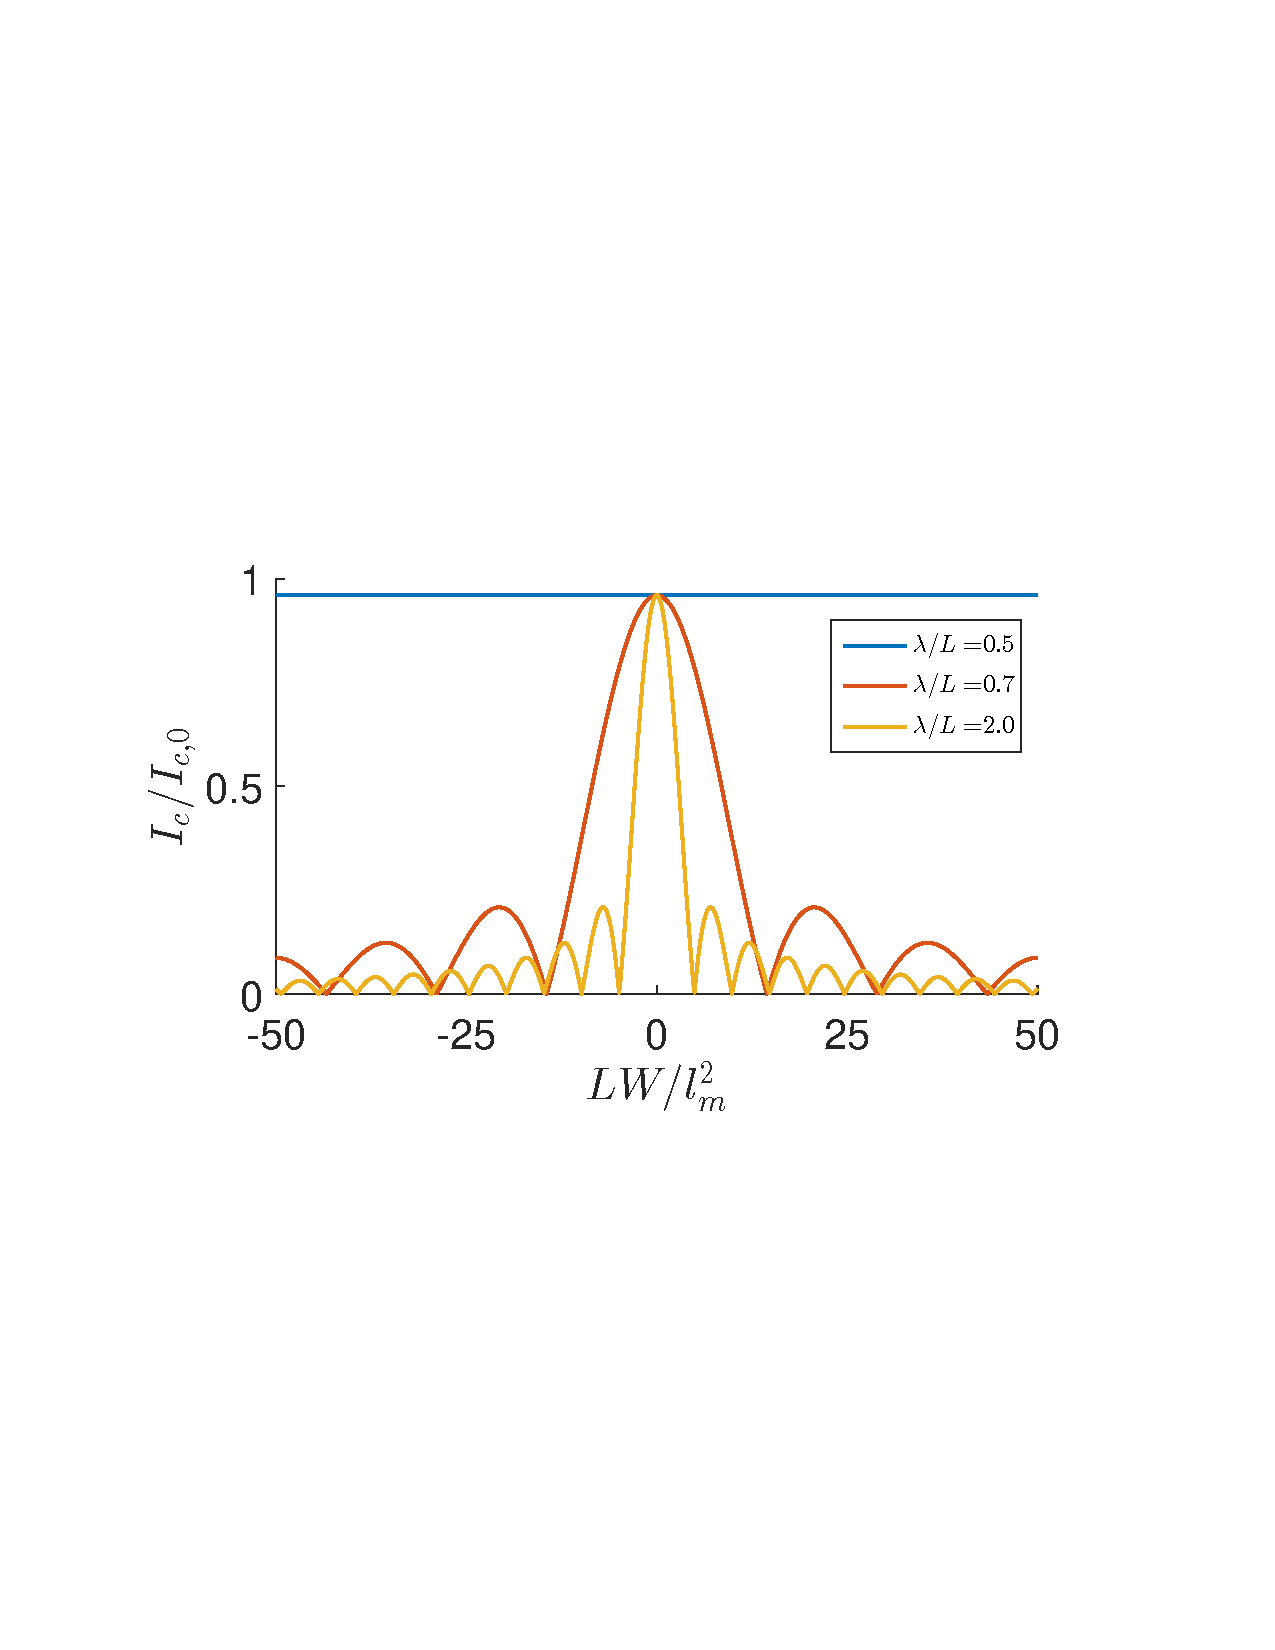
\includegraphics[width=8cm,clip=true,trim=2cm 8cm 3cm 9cm]{fig/Critical5}
%\subfigure[]{\includegraphics[width=3.9cm]{Dustin}\label{fig:Dustin}}
%\hfill
%\subfigure[]{\includegraphics[width=3.45cm]{Martin}\label{fig:Martin}}
\caption{blabla}
\label{fig:Critical5}
\end{figure}


\subsubsection{Anti-symmetric field}
Taking $\varphi$ to zero in \eqref{B4} the magnetic field becomes anti-symmetric about the $y$-axis, and the first term in \eqref{gamma2} vanishes:
\begin{equation}
\gamma = \frac{L^2}{l_m^2}\tan\theta_k\left[\left(\frac{\lambda}{\pi L}\right)^2\sin\left(\frac{\pi L}{\lambda}\right)-\frac{\lambda}{\pi L}\cos\left(\frac{\pi L}{\lambda}\right)\right].
\label{gammaDist4}
\end{equation}
We notice how $\gamma$ now is position-independent and expect a uniform current distribution without current vortices. The magnetic wavelength dependency of $\gamma$ is shown in figure \ref{fig:Gamma4}. For certain wavelengths, $\lambda$, $\gamma$ will be zero regardless of the field strength or position and we expect the current to be unaffected by the magnetic field. Using the expression for $\gamma$ \eqref{gammaDist4} in equation \eqref{dIwithB} and \eqref{CurrentDensity} the current density is found numerically and the result is shown in figure \ref{fig:Dist4} for varying wavelengths, $\lambda$, of the external field.
\begin{figure}[hhh]
\centering
%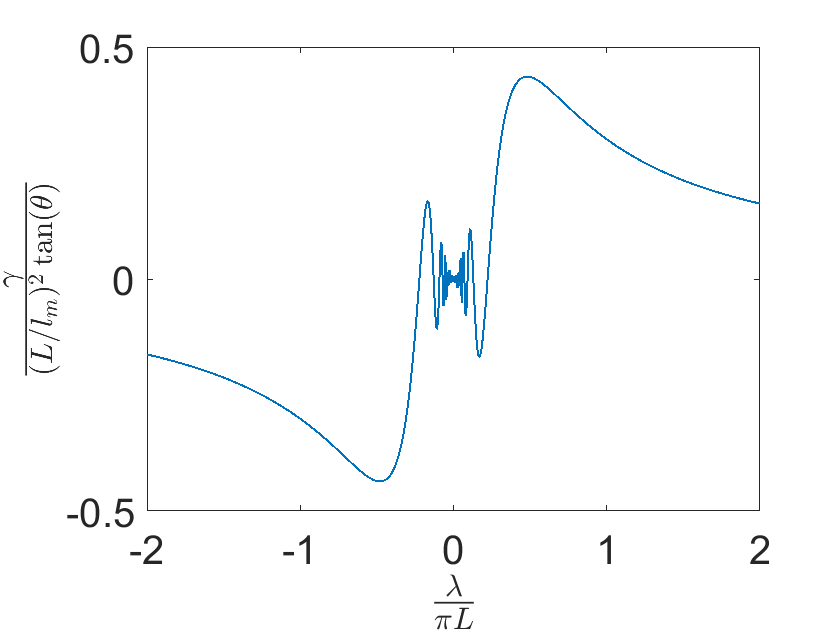
\includegraphics[width=10cm]{fig/1_Max3_l_0-3_phi_0}
\subfigure[]{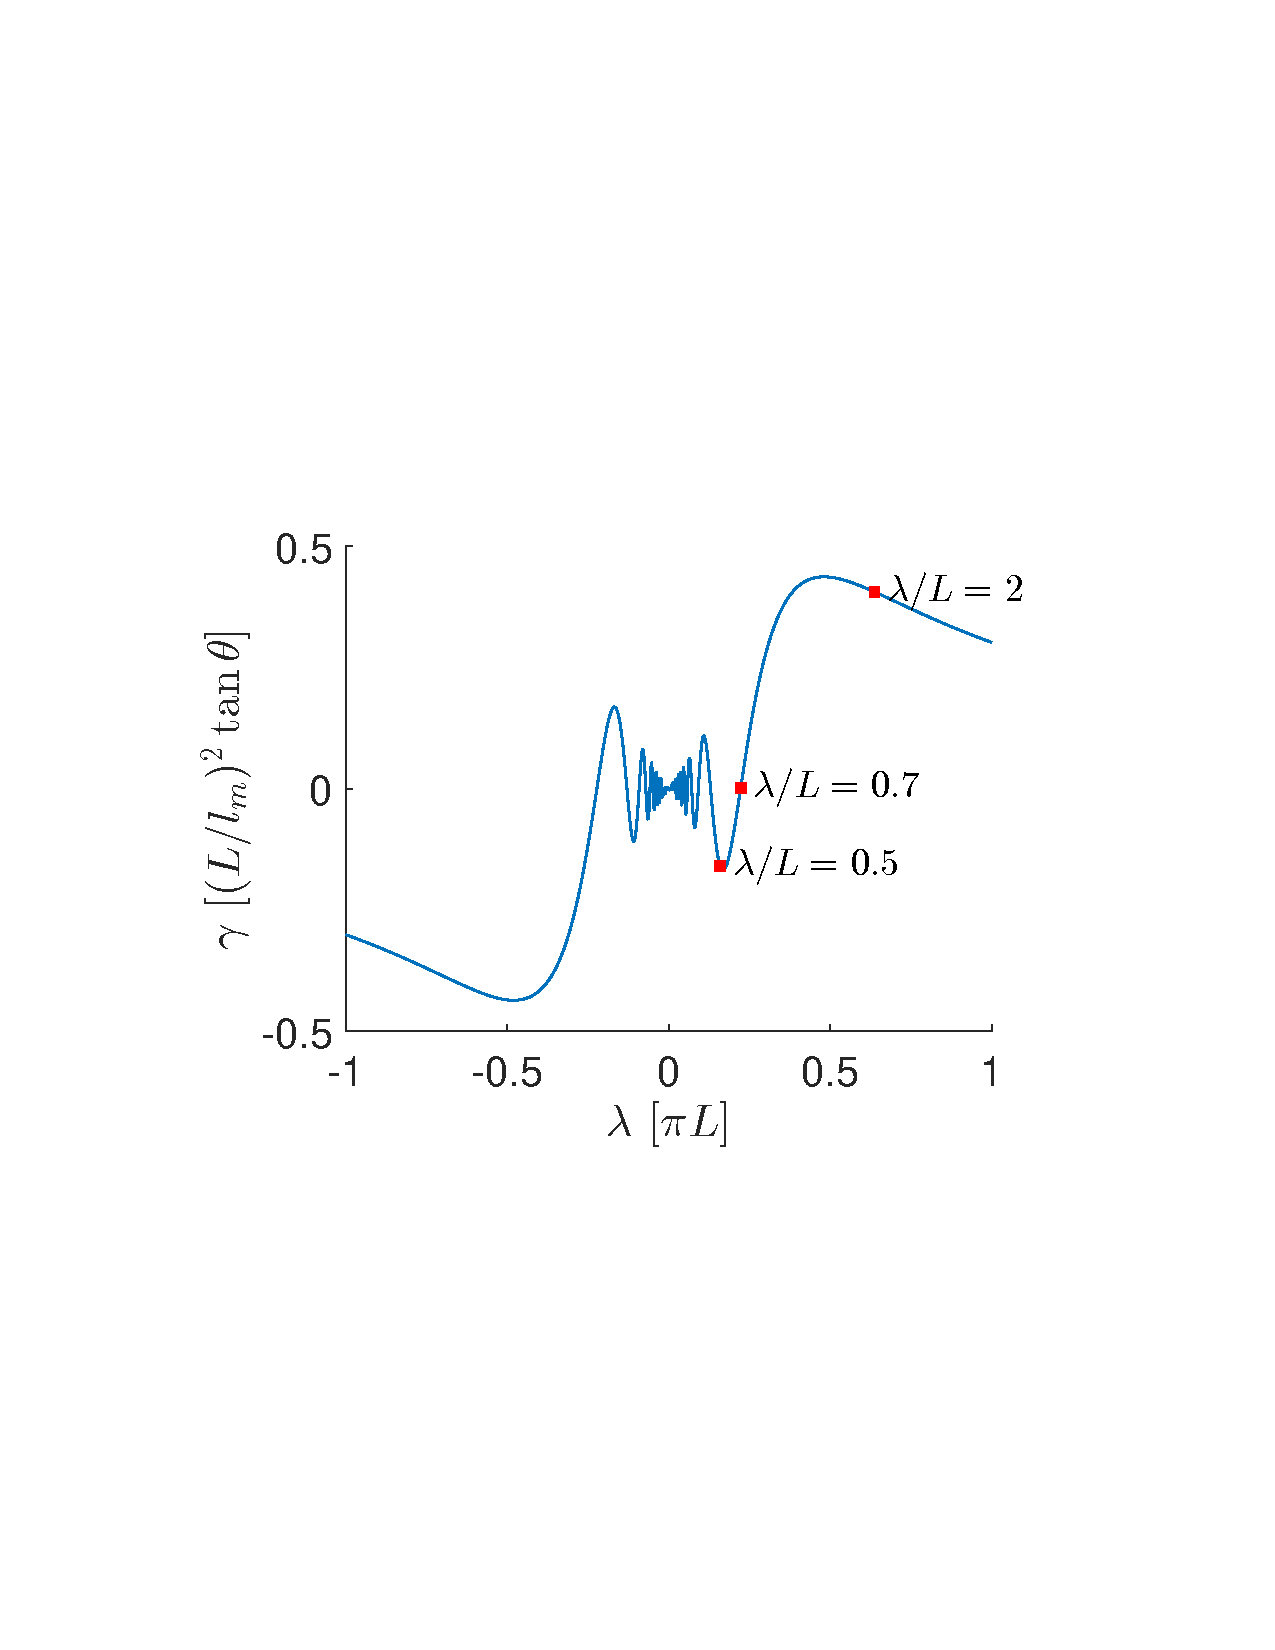
\includegraphics[width=8cm,clip=true,trim=3cm 8cm 2cm 8cm ]{fig/Gamma4}\label{fig:Gamma4}}
\hfill
\subfigure[]{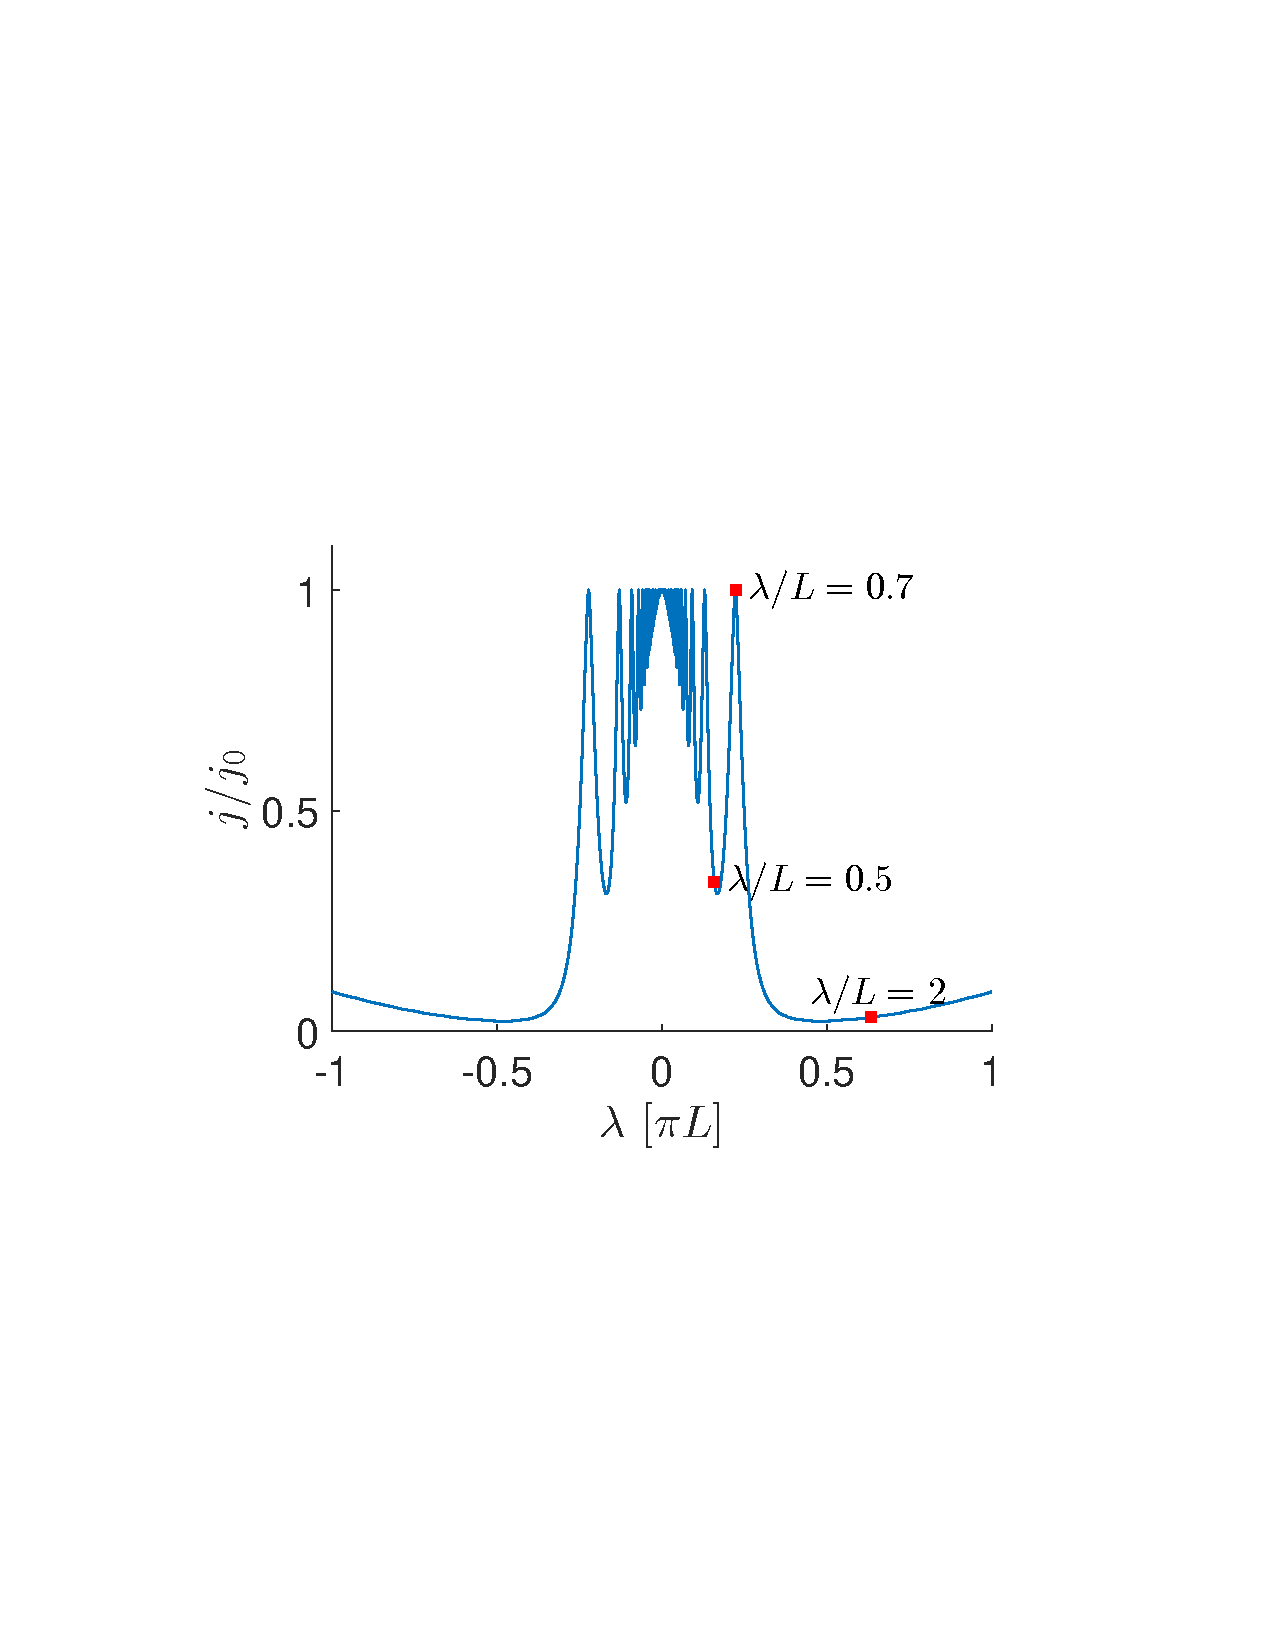
\includegraphics[width=8cm,clip=true,trim=3cm 8cm 2cm 8cm ]{fig/Dist4}\label{fig:Dist4}}
\caption{blabla}
\label{fig:motionEarth}
\end{figure}
\\
\\
We find the total current in the high temperature regime as we did for the uniform field in section \ref{sec:ConstField}. As $\gamma$ \eqref{gamma2} is independent of $y_0$, equation \eqref{TotalCurrentHighT} yields
\begin{equation}
I = \frac{I_{c,0}}{2}\int_{-\pi/2}^{\pi/2}d\theta_k\cos\theta_k\sin(\Delta \varphi - \gamma).
\end{equation}
Using that $\gamma(\theta_k) = -\gamma(-\theta_k)$ this can be rewritten to
\begin{equation}
I = I_{c,0}\sin\Delta\varphi\int_0^{\pi/2}d\theta_k\cos\theta_k\cos\gamma.
\end{equation}
After inserting for $\gamma$ and integrating over $\theta_k$ we obtain the total current,
\begin{equation}
I = I_{c,0}\sin\Delta\varphi\frac{L^2}{l_m^2}\left|f(\lambda)\right|K_1\left(\frac{L^2}{l_m^2}\left|f(\lambda)\right|\right),
\end{equation}
where $K_1(z)$ is the modified Bessel function of second kind and we have defined
\begin{equation}
f(\lambda) \equiv \left(\frac{\lambda}{\pi L}\right)^2\sin\left(\frac{\pi L}{\lambda}\right)-\frac{\lambda}{\pi L}\cos\left(\frac{\pi L}{\lambda}\right).
\end{equation}
Hence, the high temperature critical current is
\begin{equation}
    I_c = I_{c,0}\frac{L^2}{l_m^2}\left|f(\lambda)\right|K_1\left(\frac{L^2}{l_m^2}\left|f(\lambda)\right|\right).
\label{Critical4}
\end{equation}
The wavelengths $\lambda$ that make $f(\lambda)$ go to zero, will give $I_c = I_{c,0}$, regardless of the magnetic field strength. In figure \ref{fig:Critical4} the critical current obtained from numerical computation is shown for different wavelengths, $\lambda$, and varying magnetic field strength, $B$. This result is in correspondance with the analytical expression \eqref{Critical4}. We notice that we no longer have the familiar Fraunhofer pattern and understand this as being a consequence of the absence of the current vortices. Just like we found for the symmetric field there exists wavelengths, e.g. $\lambda \approx 0.7 L$, which make the critical current $I_c$ remain constant when the magnetic field strength increases.

\subsection{Sinusoidal field varying along the interfaces}
\label{sec:alongInterface}
Instead of varying the field along the junction we will now consider a sinusoidal magnetic field varying along the interfaces:
\begin{equation}
    \fet{B} = B\sin\left(\frac{2\pi}{\lambda}y + \varphi\right)\left[\Theta(x+L/2) - \Theta(x-L/2) \right]\hat{z}
\label{Binterface}
\end{equation}
with the gauge
\begin{equation}
    \fet{A} = B\frac{\lambda}{2\pi}\cos\left(\frac{2\pi}{\lambda}y+\varphi\right)\left[\Theta(x+L/2) - \Theta(x-L/2) \right]\hat{x}.
\end{equation}
Now the phase shift becomes
\begin{equation}
\begin{split}
    \gamma &= 
    %\frac{2}{l_m^2}\frac{\lambda}{2\pi}\int \cos\left(\frac{2\pi}{\lambda}y(x) + \varphi \right) dx =
    %\frac{\lambda}{\pi l_m^2 \tan\theta_k}\int_{y_L}^{y_R} \cos\left(\frac{2\pi}{\lambda}y + \varphi \right) dy
    %\\&= 
    -\frac{\lambda^2}{l_m^2\pi^2\tan\theta_k}\sin\left(\frac{\pi L}{\lambda}\tan\theta_k\right)\cos\left(\frac{2\pi}{\lambda}\left[y_0-x_0\tan\theta_k\right] + \varphi\right).
\end{split}
\end{equation}
%where $y_L$ is the $y$-component of the starting position of the trajectory \eqref{trajectory} in the left superconductor, while $y_R$ is the $y$-component of the end position in the right superconductor. 
As we did in the previous section we will also here look at the symmetric- and anti-symmetric fields taking $\varphi$ to $\pi/2$ and $0$, respectively.

\subsubsection{Symmetric field}
In the  symmetric field, i.e. when $\varphi =\pi/2$ the phase shift is
\begin{equation}
\begin{split}
    \gamma &= -\frac{\lambda^2}{l_m^2\pi^2\tan\theta_k}\sin\left(\frac{\pi L}{\lambda}\tan\theta_k\right)\sin\left(\frac{2\pi}{\lambda}\left[y_0-x_0\tan\theta_k\right]\right). 
    \\
    &= -\gamma_{\mathrm{uni}}\frac{\sin\left(\frac{\pi L}{\lambda}\tan\theta_k\right)}{\frac{\pi L}{\lambda}\tan\theta_k}\frac{\sin\left(\frac{2\pi}{\lambda}\left[y_0-x_0\tan\theta_k\right]\right)}{\frac{2\pi}{\lambda}\left[y_0-x_0\tan\theta_k\right]},
\end{split}
\label{Gamma3}
\end{equation}
where $\gamma_{\mathrm{uni}}$ is the phase shift in the uniform field. In the limit with $\lambda \gg L$ and $\lambda \gg y_0$ the phase shift will approach the phase shift in the uniform field, $\gamma \rightarrow -\gamma_{\mathrm{uni}}$, as we would expect as a symmetric magnetic field will be approximately constant when the wavelength becomes very large. In the limit with $\lambda \ll L$ the second factor in \eqref{Gamma3} will go to zero and the current density will be as if there was no magnetic field present. 
\\
\\
In order to compare this field with the uniform field we consider the current density at $x_0=0$ and $\theta_k = 0$ in which the phase shift is
\begin{equation}
    \gamma(x_0=0,y_0,\theta_k=0) = -\gamma_{\mathrm{uni}}\frac{\sin\left(\frac{2\pi}{\lambda}y_0\right)}{\frac{2\pi}{\lambda}y_0}.
    %= -\gamma_{\mathrm{uni}}(y_0-\lambda/4)\frac{\cos\left(\frac{2\pi}{\lambda}\left(y_0-\frac{\lambda}{4}\right)\right)}{\frac{2\pi}{\lambda}\left(y_0-\frac{\lambda}{4}\right)}
\end{equation}
Compared to the phase shift in the uniform field we have now an additional factor which will envelope the vortex rows we saw in the uniform field with a periodicity $\lambda$. The current density pattern will in this case depend on the phase difference $\Delta \varphi$, unlike what we have seen in the fields so far considered. We will consider two specific cases, namely $\Delta \varphi = n\pi$ and $\Delta \varphi = (n+1/2)\pi$, in which the the current density along the $y$-axis will be an even or odd function of $\gamma$, respectively, according to equation \eqref{dIwithBHighT}. When the current density is an odd function of $\gamma$ we expect the vortex-antivortex rows for the uniform field to be repeated as rows and anti-rows of vortices with row lattice constant $a_{\mathrm{row,odd}} = \lambda$. When the current density is an even function of $\gamma$ we expect the vortex rows to be separated by a row lattice constant $a_{\mathrm{row,even}} = \lambda/2$. Moreover, as the factor $\sin(2\pi y_0/\lambda)/(2\pi y_0/\lambda)$ is an even function of $y_0$ we expect the vortex rows to be symmetric about the $x$-axis, even when the current density is an odd function of $\gamma$. That is the pattern is such that if a row is placed at $y_0$ then there is a corresponding row placed at $-y_0$.
\\
\\
The current density is found numerically from equation \eqref{dIwithB} and \eqref{CurrentDensity} and the result is shown in figure \ref{fig:Dist3} for different wavelengths. We observe what was predicted, namely a repeated pattern of vortex-anti-vortex-rows. With $\Delta \varphi = 0$ we observe rows and anti-rows separated by $\lambda/2$ such that each row is separated by $\lambda$, i.e. row lattice constant $a_{\mathrm{row,odd}}=\lambda$. With $\Delta \varphi = \pi/2$ there are no anti-rows as the current density is an even function of $\gamma$ and each row is separated by $\lambda/2$, i.e. row lattice constant $a_{\mathrm{row,even}}=\lambda/2$. Moreover, the current density approaches a uniform distribution as $\lambda \rightarrow 0$ with current as given in equation \eqref{WithoutField}, as we predicted analytically. When $\lambda >> L$ the uniform field pattern reappears, as predicted. 
\begin{figure}[hhh]
\centering
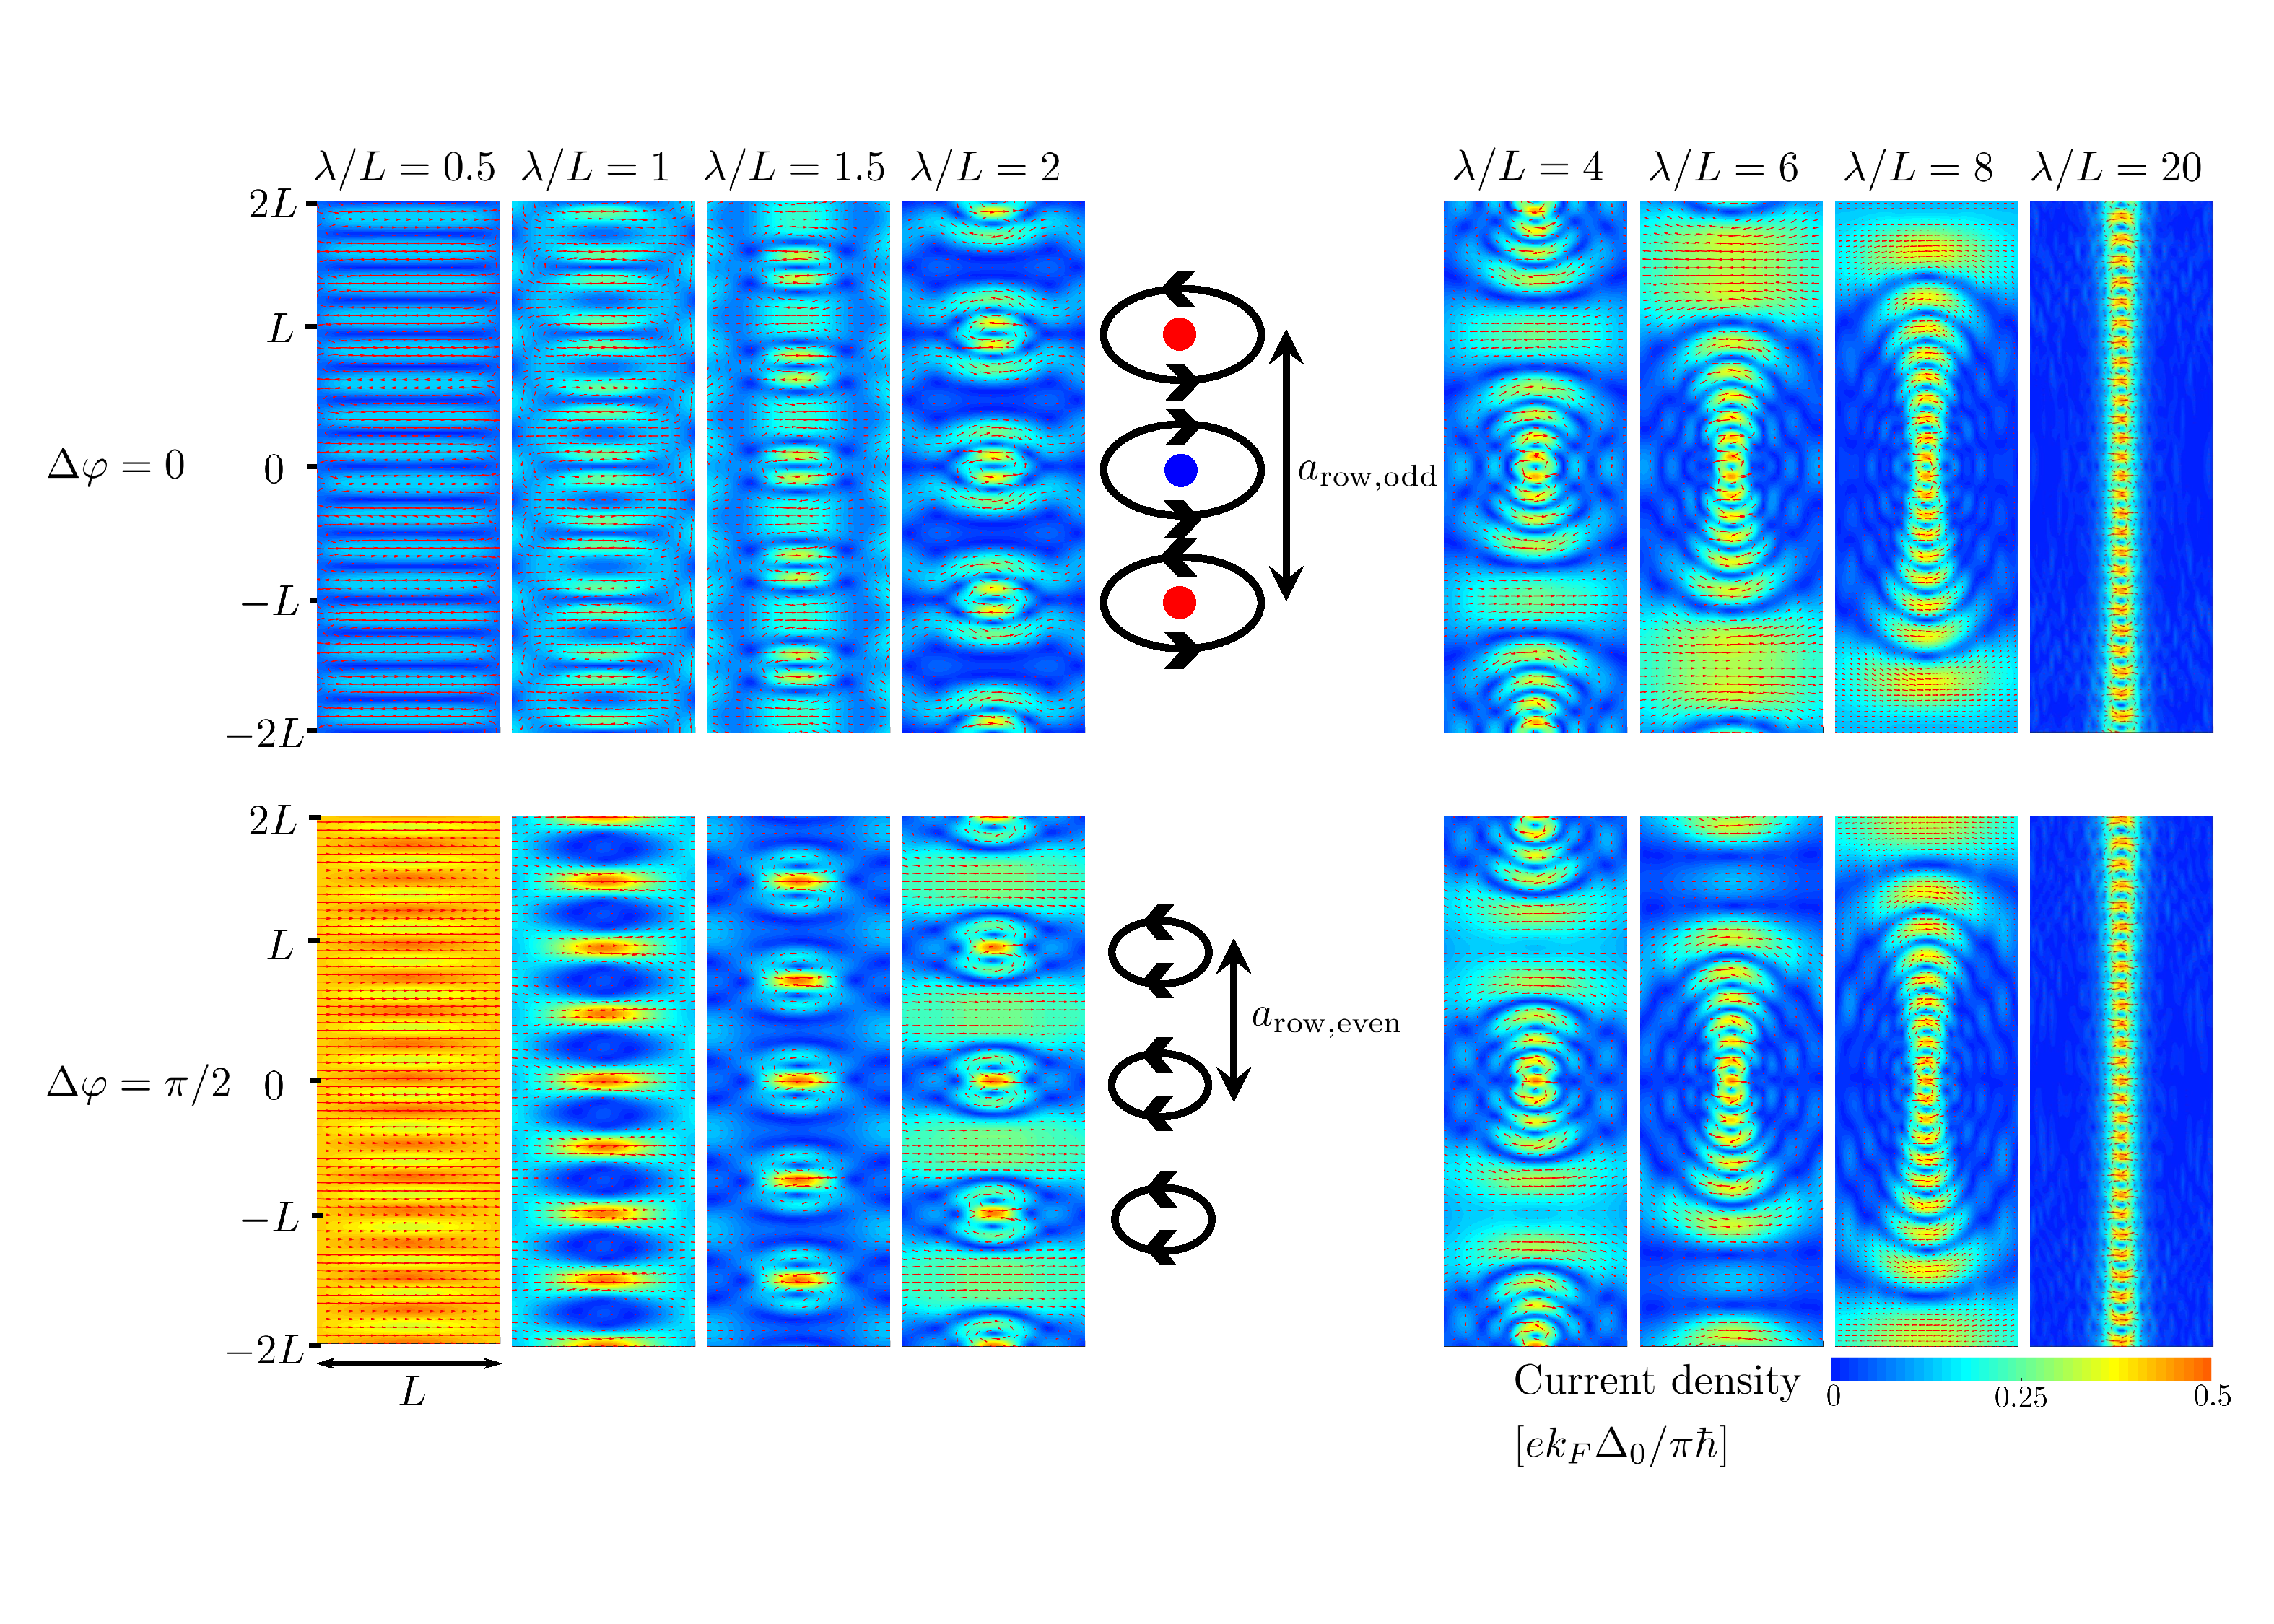
\includegraphics[width=17cm,clip=true,trim = 0cm 3.5cm 0cm 3cm]{fig/Dist3}
\caption{blabla.. Planen her å gjøre figurene litt finere sånn som for konstant felt. Og vise to rader med bilder, en med $\Delta \varphi = 0$ og en med $\Delta \varphi = \pi/2$}
\label{fig:Dist3}
\end{figure}
As the expression for $\gamma$ is quite complicated we can not calculate the total current analytically, even in the high temperature regime. However, the critical current is found numerically and the result is shown in figure \ref{fig:Critical2}. For large wavelengths, $\lambda$, the critical current approaches the Fraunhofer pattern as we would expect from the results found in the current density. Moreover, the critical current smoothens out and approaches the constant critcal current $I_{c,0}$ when the wavelength goes to zero.
\begin{figure}[hhh]
\centering
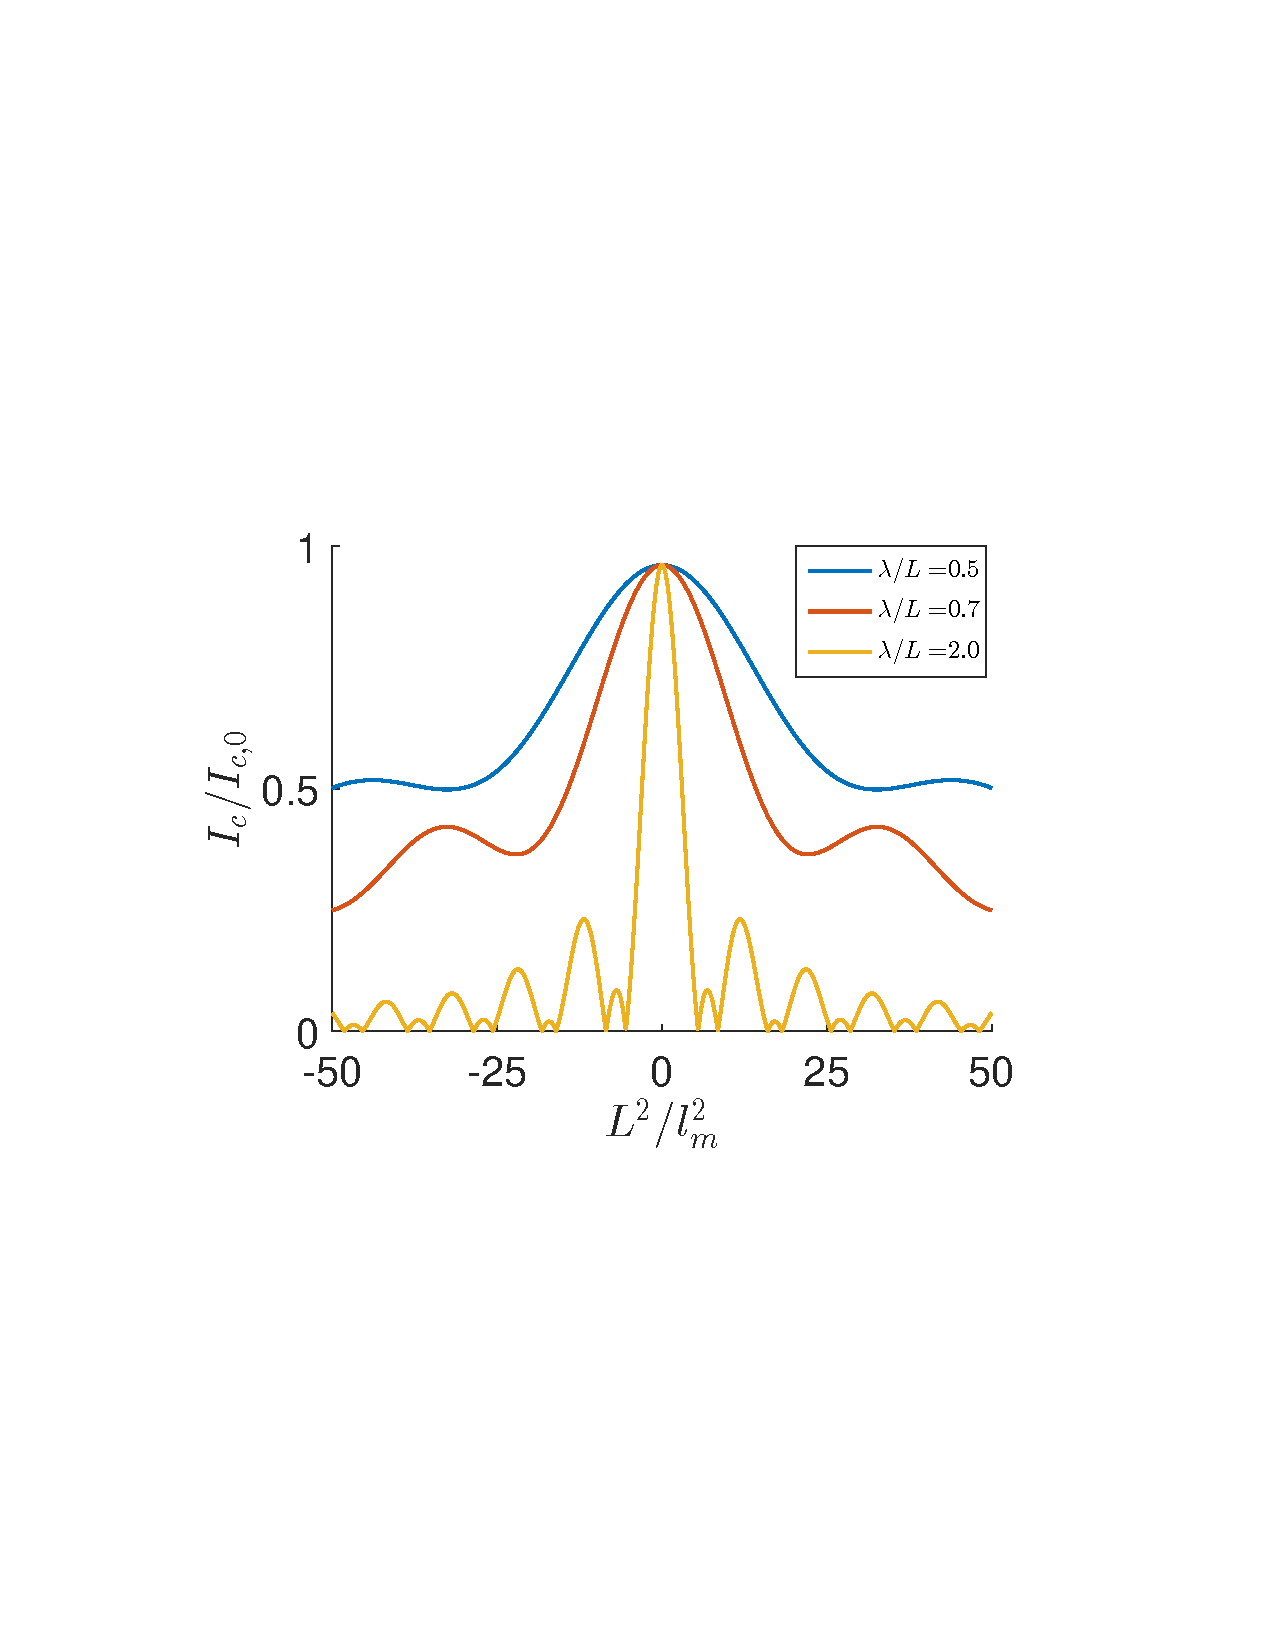
\includegraphics[width=8cm,clip=true,trim=3cm 8cm 4cm 9cm]{fig/Critical2}
\caption{blabla}
\label{fig:Critical2}
\end{figure}


\subsubsection{Anti-symmetric field}
We now let $\varphi = 0$ such that the magnetic field is anti-symmetric about the $x$-axis with the phase shift
\begin{equation}
\begin{split}
    \gamma &= -\frac{L^2}{l_m^2}\frac{\lambda}{\pi L }\frac{\sin\left(\frac{\pi L}{\lambda}\tan\theta_k\right)}{\frac{\pi L}{\lambda}\tan\theta_k}\sin\left(\frac{2\pi}{\lambda}\left[\left(y_0+\frac{\lambda}{4}\right)-x_0\tan\theta_k\right]\right)\\
    %&=-\frac{L^2}{l_m^2}\frac{\lambda}{\pi L }\frac{\sin\left(\frac{\pi L}{\lambda}\tan\theta_k\right)}{\frac{\pi L}{\lambda}\tan\theta_k}\cos\left(\frac{2\pi}{\lambda}\left[y_0-x_0\tan\theta_k\right]\right)\\
    %&=-\gamma_{\mathrm{uni}}(x_0,y_0,\theta_k)\frac{\sin\left(\frac{\pi L}{\lambda}\tan\theta_k\right)}{\frac{\pi L}{\lambda}\tan\theta_k}\frac{\cos\left(\frac{2\pi}{\lambda}\left[y_0-x_0\tan\theta_k\right]\right)}{\frac{2\pi}{\lambda}\left[y_0-x_0\tan\theta_k\right]}\\
    %&=-\gamma_{\mathrm{uni}}\left(x_0,y_0+\frac{\lambda}{4},\theta_k,\right)\frac{\sin\left(\frac{\pi L}{\lambda}\tan\theta_k\right)}{\frac{\pi L}{\lambda}\tan\theta_k}\frac{\sin\left(\frac{2\pi}{\lambda}\left[\left(y_0+\frac{\lambda}{4}\right)-x_0\tan\theta_k\right]\right)}{\frac{2\pi}{\lambda}\left[\left(y_0+\frac{\lambda}{4}\right)-x_0\tan\theta_k\right]}\\
\end{split}
\end{equation}
This is equal to the symmetric field \eqref{Gamma3}, only shifted by $\lambda/4$ along the $y$-axis. Hence we expect a similar, but shifted pattern as for the symmetric case. At $\theta_k = 0$ and $x_0 = 0$ the phase shift is 
\begin{equation}
    \gamma(x_0=0, y_0, \theta_k = 0) = -\gamma_{\mathrm{uni}} \frac{\cos\left(\frac{2\pi}{\lambda}y_0\right)}{\frac{2\pi}{\lambda}y_0}.
\end{equation}
The factor $\cos(2\pi y_0/\lambda)/(2\pi y_0 /\lambda)$ is an odd function of $y_0$ and unlike the symmetric case we now expect an anti-symmetric pattern about the $x$-axis if the current is an odd function of $\gamma$, i.e. when $\Delta \varphi = n\pi$. That is if there is a row placed at $y_0$ there will be a anti-row placed at $-y_0$. This is confirmed numerically and the result is shown in figure \eqref{fig:Dist2}.
\begin{figure}[hhh]
\centering
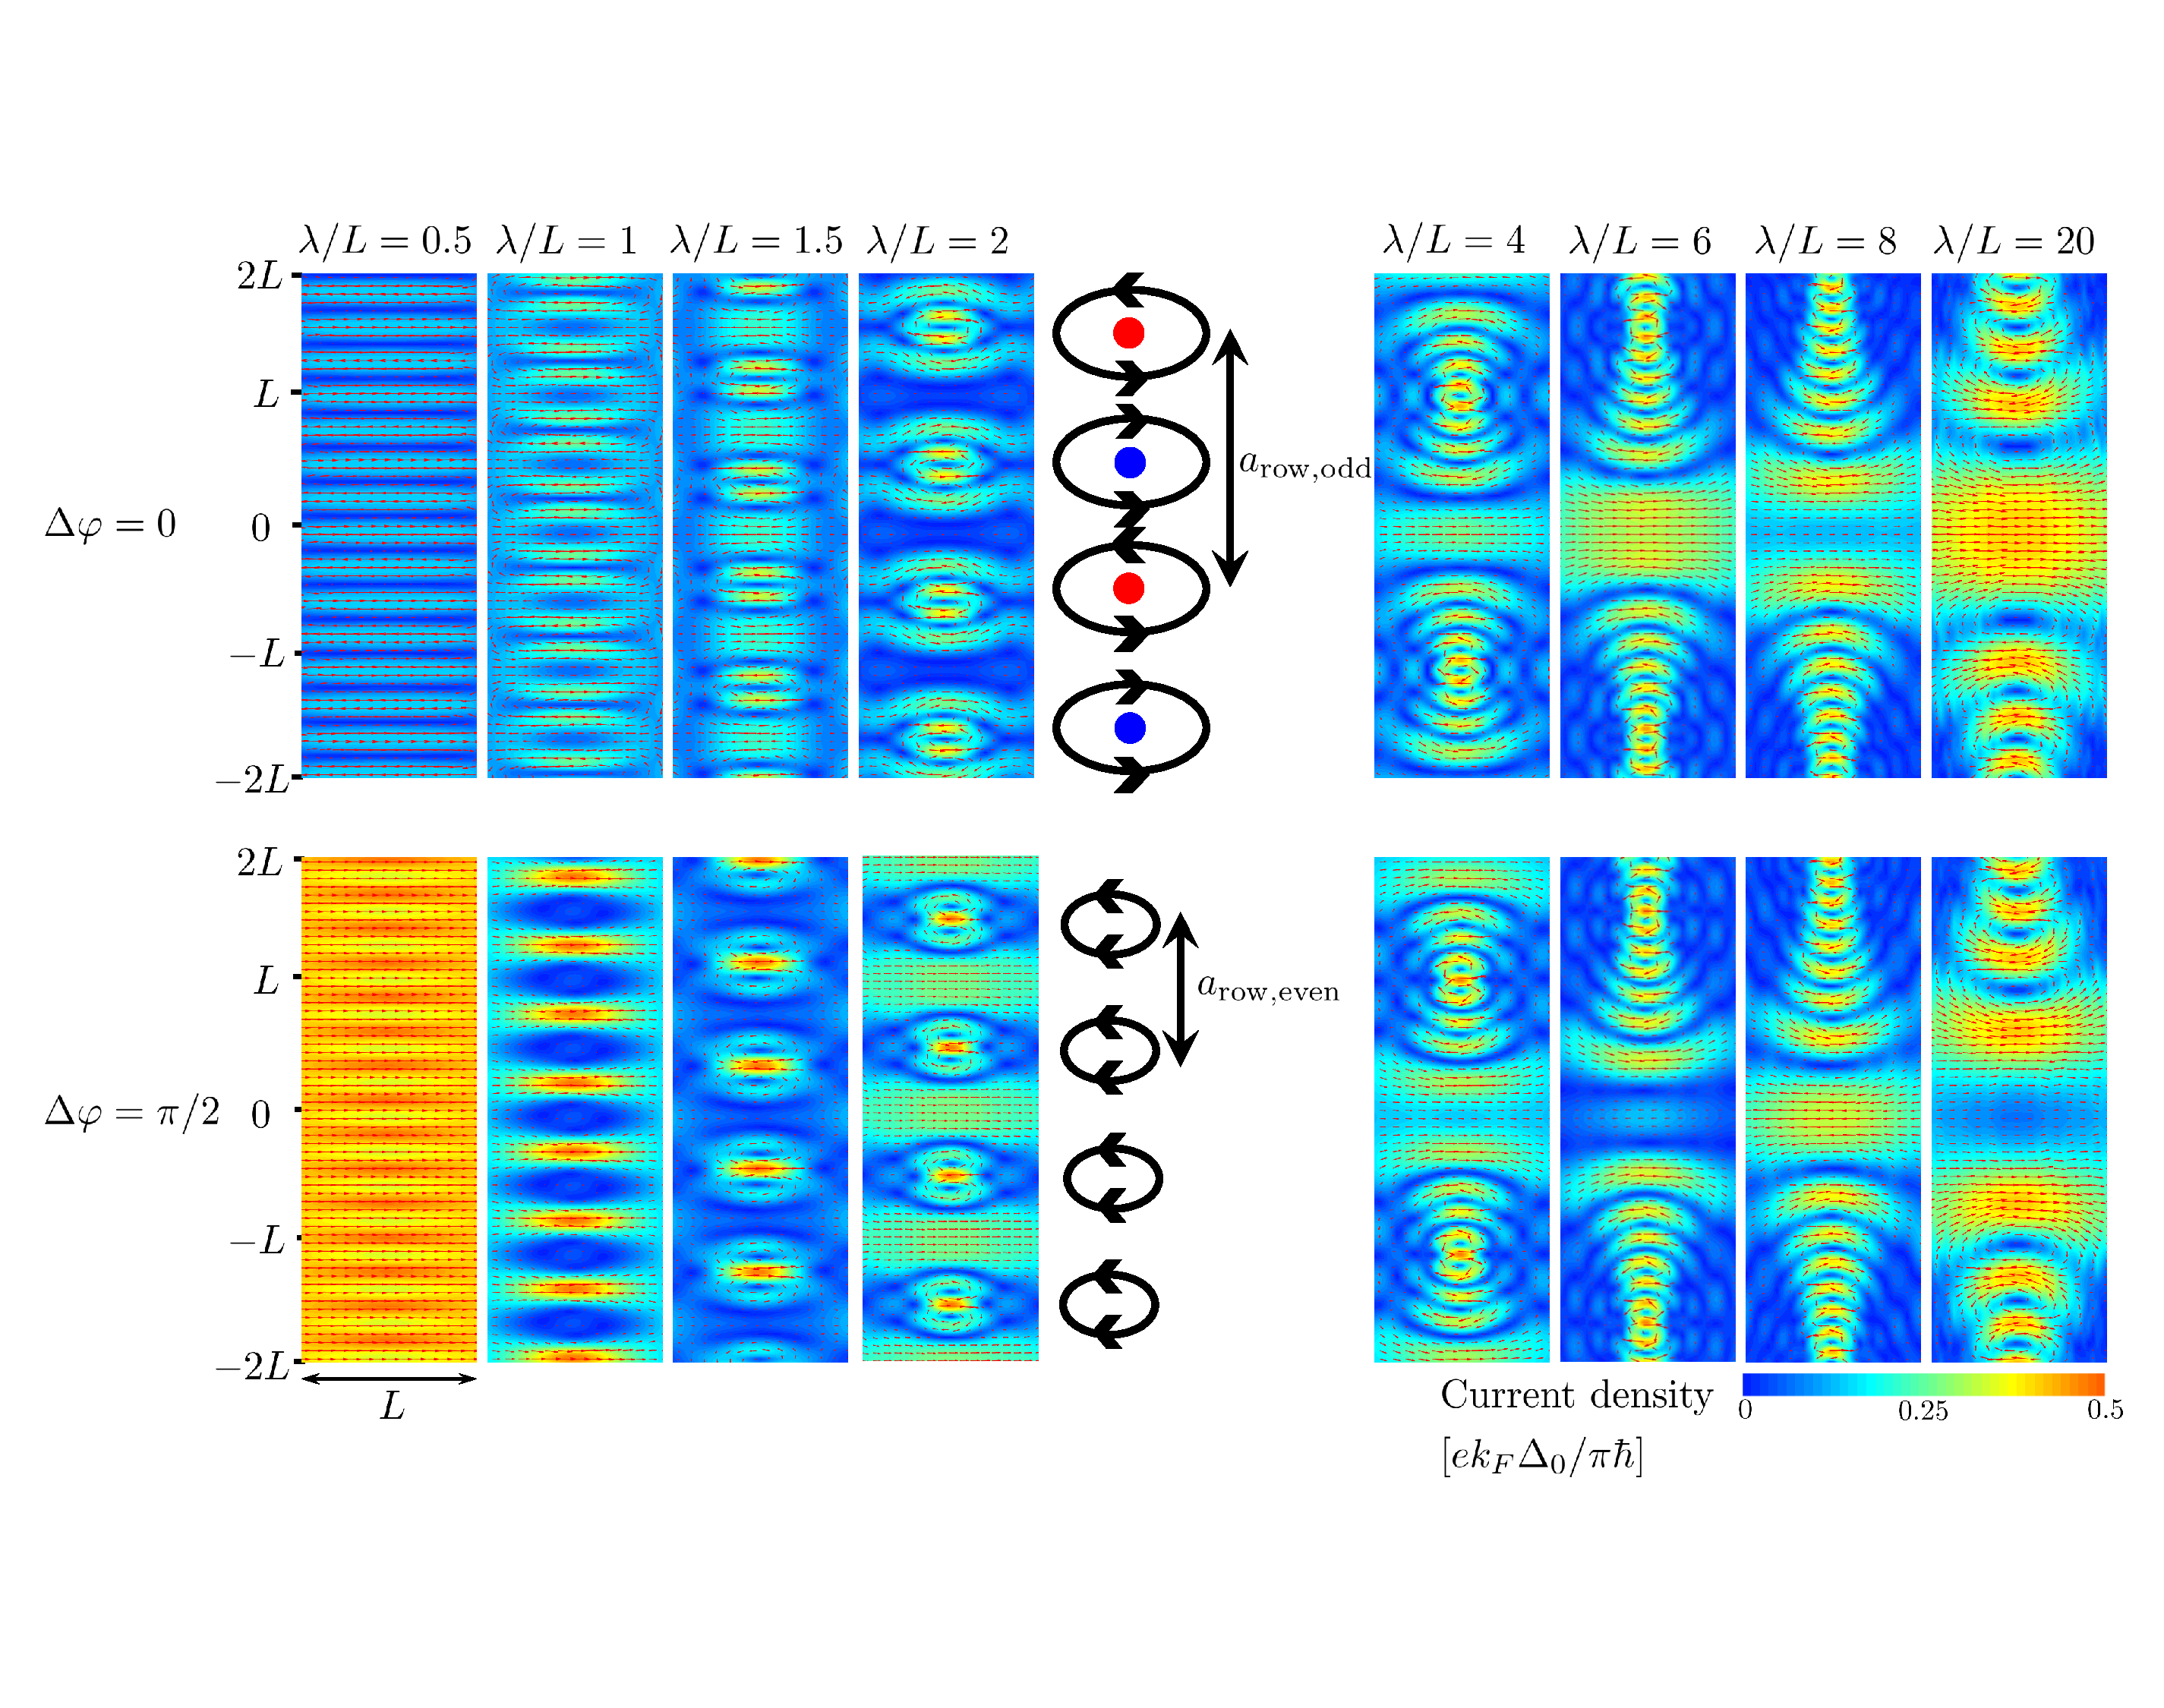
\includegraphics[width=17cm,clip=true,trim = 0cm 5cm 0cm 2cm]{fig/Dist2}
\caption{blabla.. Planen her å gjøre figurene litt finere sånn som for konstant felt. Og vise to rader med bilder, en med $\Delta \varphi = 0$ og en med $\Delta \varphi = \pi/2$}
\label{fig:Dist2}
\end{figure}
\\
\\
Since the current density of the symmetric and anti-symmetric field along the interface only differ by a shift of the center of the vortex rows along the $y$-axis, we expect the total current to be equal in the two cases, when $W \gg L$. This has also been confirmed numerically, and the critical current will be as shown in figure \ref{fig:Critical2}.